\documentclass[12pt,b5paper]{book}
\usepackage[toc,page]{appendix}
\usepackage[utf8]{inputenc}
\usepackage{csquotes}
\usepackage{fullpage}
\usepackage[english]{babel}
\usepackage{amsmath}
\usepackage{amsthm}
\usepackage{amsfonts}
\usepackage{amssymb}
\usepackage{graphicx}
\usepackage{listings}
\usepackage{paralist}
\usepackage{tikzsymbols}
\lstset{frame=lrbt}
\lstset{basicstyle=\footnotesize}

\lstset
{
	basicstyle=\scriptsize\ttfamily,
	breaklines=true,
	frame=single,
	showstringspaces=false,
	tabsize=2
}

\theoremstyle{definition}
\newtheorem{example}{Example}

\title{Friendly F\# - fun with logic.}
\author{Dr. Giuseppe Maggiore \\
Dr. Giulia Costantini \\
Francesco Di Giacomo \\
Gerard van Kruiningen}

\begin{document}
\maketitle
\tableofcontents

\chapter{Introduction}
\label{sec:introduction}
The goal of this document is to make you acquainted with the concept of inference systems. You will learn various aspects of logic and inference system, which we will use to give rise to definitions of concepts such as numbers, boolean expressions, etc. As an advanced example you will also learn how to model programming languages constructs into inference systems. This leads to an important end result: you will learn the \textit{what} of programming languages, in contrast to the \textit{how} that you have studied so far. As a short conclusion we will discuss the strong relationship between logic and programming, and draw some conclusions about computability.

\subsection{Why bother?}
Try drawing a circle or a similar shape. The circle starts out as a single ``piece''. Choose two points along the border and draw a connecting line between the two: the circle is now split into two pieces. Chose now a third point and connect it to the other two points: the circle is now split into four pieces. A clear pattern is emerging: every point we add, we get twice as many pieces. This suggests that by \texttt{k} points we get $2^{k-1}$ pieces.

This seems all quite logical, but there is a catch. Try now doing this with six points along the border of the circle: instead of the expected 32 pieces, we will end up with 31. This means that the original conclusion was definitely not correct.

What is the moral of this story? If you want (or need) to be absolutely sure about some assertion (often called \textit{proposition} or \textit{hypothesis}), then you cannot trust a few examples and an intuitively appealing story to show that some pattern will always hold true. In the practice, and certainly in that of informatics or medical technology, there are many situations where a few tests and an intuition of why the system works are sufficient. Would you dare fly in an airplane where the programmer concluded after a dozen of tests that ``it all works, send it to production''? Would you dare step into an MRI machine (which throws radioactive isotopes at your body) knowing that the software was quickly written during a weekend with a bit of unit testing? Of course not\footnote{as a side note, if you are comfortable with these scenarios, then perhaps the motivation for the rest of the document will feel quite weak, so you might better go back to your vacation in Chernobyl or flying in planes held together by duct tape.}.

The use of logic as a foundation for programming does not automatically solve all our problems. It is very well possible (we will get there) that there is no single mathematical formalism or piece of software that will entirely remove the need for human intellect when writing software. \textbf{In any case, the use of logic and formality when decomposing problems can greatly help in writing software that is better thought out and over which it is far easier to reason and prove properties.}

\subsection{Structure of the document}
In the rest of this document we will: 
\begin{inparaenum}[\itshape i\upshape)]
\item introduce informal logical reasoning in Section \ref{sec:informalIntroduction};
\item introduce a more formal logical formalism in Section \ref{sec:inferenceSystems};
\item give a first example of logic in action to define basic boolean operators in Section \ref{sec:booleanExpressions};
\item use logic to define \textit{apparently atomic} and unrelated concepts such as numbers in Chapter \ref{chap:numbers};
\item construct complex data structures such as lists, binary search trees, and even balanced binary search trees in Chapter \ref{chap:dataStructures};
\item build a small programming language in Chapter \ref{chap:aPL};
\item we conclude with a short and woefully incomplete presentation of fragments of computability in Chapter \ref{chap:closingRemarks}.
\end{inparaenum}



\section{An informal introduction to logic}
\label{sec:informalIntroduction}
The basic rules of logic are very simple. Logica is entirely defined as a way to manipulate symbols. These symbols are usually common signs such as numbers, letter, Greek letters, etc., but it is not forbidden to use any symbol we find useful or interesting. In this section, precisely with the goal of illustrating the \textit{independence of logic from the symbols chosen}, we shall manipulate smileys and other icons. \textbf{The first step is thus choosing the symbols.} Logic is really the description of most (complex) dynamic processes that search for an answer in a complex space. This search may be a purely mathematical search, or it could be a program running. The dynamic process is defined in terms of a series of rules which are activated whenever we find a matching input. Thus, \textbf{the second step is choosing the rules that define our dynamic processes}.

After defining symbols and rules, things become interesting and we can try to use our system to find answers and process information. We usually start with a given proposition, which is the input of the whole process. A \textit{proposition} is just a series of symbols, such as for example: \texttt{3 + 2 = 5 of \dSmiley\dSmiley\Candle\Candle}. We apply the rules to the proposition until we reach the desired answer, and we have also answered all of the intermediate questions that came to existance during the dynamic process.

\paragraph{A concrete example}
Let us consider a full example. Consider the symbols of our language to be:
\begin{itemize}
\item A smiley \dSmiley
\item A candle \Candle
\item A tree \Springtree
\item A coffee cup \Coffeecup
\end{itemize}

We consider a proposition to be true if and only if we can process it until we reach a \Coffeecup. \footnote{Given the extreme importance of coffee in the diet of mathematicians and computer scientists, equating coffee with truth does not really seem that illogical a step} Our rules are:

\begin{itemize}
\item \textbf{(G0)} A \Coffeecup means we are done
\item \textbf{(R1)} Two \dSmiley followed by a \Springtree, and then further followed by \texttt{r}, means that we will have to process \texttt{r} to find the answer
\item \textbf{(R2)} Two \Candle followed by a \Springtree, and then further followed by \texttt{r}, means that we will have to process \texttt{r} to find the answer
\end{itemize}

Consider now the input proposition of \\
\dSmiley\dSmiley\Springtree\Candle\Candle\Springtree\dSmiley\dSmiley\Springtree\Coffeecup \\

We begin by using \textbf{R2}, therefore obtaining: \\
\Candle\Candle\Springtree\dSmiley\dSmiley\Springtree\Coffeecup \\

We then use rule \textbf{R1}, therefore obtaining: \\
\dSmiley\dSmiley\Springtree\Coffeecup \\

We then use rule \textbf{R2}, therefore obtaining: \\
\Coffeecup \\

Now according to \textbf{G0} we are done. The proof is successfull, therefore we can conclude that \dSmiley\dSmiley\Springtree\Candle\Candle\Springtree\dSmiley\dSmiley\Springtree\Coffeecup was \textbf{true within our system of rules}. 

Consider now the new input proposition of \\
\dSmiley\dSmiley\Springtree\dSmiley\dSmiley\Springtree\Candle\Springtree\Coffeecup \\

We begin by using \textbf{R2}, therefore obtaining: \\
\dSmiley\dSmiley\Springtree\Candle\Springtree\Coffeecup \\

We then use rule \textbf{R1}, therefore obtaining: \\
\Candle\Springtree\Coffeecup \\

Unfortunately now we cannot apply rule \textbf{R1} again, because we have no \dSmiley at the head of our proposition; we cannot apply rule \textbf{R2} because we have no \Candle at the head of our proposition; and we can certainly not apply rule \textbf{G0} because there is no lonely \Coffeecup. If we cannot apply any of our rules, the process is \textit{stuck}. This means that we cannot prove \dSmiley\dSmiley\Springtree\dSmiley\dSmiley\Springtree\Candle\Springtree\Coffeecup with our rules, thus \dSmiley\dSmiley\Springtree\dSmiley\dSmiley\Springtree\Candle\Springtree\Coffeecup was \textbf{not true within our system of rules}.



\section{Inference systems}
\label{sec:inferenceSystems}
In this section we present a slightly more formal treatment of inference systems. Moreover, we give a clearer syntax for expressing operators and rules. The formalism which we will use, which is also a programming language, is \textit{Meta-Casanova}. Meta-Casanova falls under the broader category of \textit{logic programming languages}, but given its structure and some of its applications it can also be considered a \textit{meta-compiler}.


\subsection{Syntax for symbol definitions}
Defining symbols in Meta-Casanova requires drawing a distinction: some symbols are considered \textit{data}, that is they are just a way to structure information, while other symbols are considered \textit{functions}, that is they are a way to define transformations from propositions to propositions.

\paragraph{Data symbols}
Data symbols are defined with the following syntax:

\begin{lstlisting}[mathescape=true]
Data [$\alpha_1$] "$\alpha_2$" [$\alpha_3$] Priority $\alpha_4$ Type $\alpha_5$
\end{lstlisting}

The $\alpha_i$'s are the arguments of the symbols:
\begin{description}
\item[$\alpha_1$] are the arguments that come left of the symbol
\item[$\alpha_2$] is the name of the symbol
\item[$\alpha_3$] are the arguments that come right of the symbol
\item[$\alpha_4$] is the priority of the symbol
\item[$\alpha_5$] is the type of the symbol
\end{description}

Examples of such a definition could be:

\begin{lstlisting}
Data [] "TRUE" [] Priority 10000 Type Expr
Data [Expr] "|" [Expr] Priority 10 Type Expr
\end{lstlisting}

the above come from the boolean expressions sample, which will be discussed in depth in a further chapter. The first line defines the \texttt{TRUE} symbols, which has no arguments left or right (it is just a value), has a very high priority (which does not matter given that this symbol has no parameters), and which is of type \texttt{Value}. The second line defines an \textit{or}-style operator that takes an \texttt{Expr} to the left, an \texttt{Expr} to the right, has a priority of 10, and is an expression itself. 

With the definitions above we can write a proposition such as \texttt{TRUE | TRUE}, which would be perfectly valid. Associativity is by default to the right, thus \texttt{TRUE | TRUE | TRUE} is equivalent to \texttt{TRUE | (TRUE | TRUE)}. We can modify the default associativity by adding a last parameter of:

\begin{lstlisting}
Data [Expr] "|" [Expr] Priority 10 Type Expr Associativity Left
\end{lstlisting}

We might even go as fast as wanting to re-define \texttt{TRUE} to a new type, because indeed we could say that \texttt{TRUE} is more a value than an expression:

\begin{lstlisting}
Data [] "TRUE" [] Priority 10000 Type Value
\end{lstlisting}

With the above definition it becomes impossible to write expressions such as \texttt{TRUE | TRUE}: the compiler will refuse this as invalid code, because \texttt{|} expects arguments of type \texttt{Expr} but it is instead given arguments of type \texttt{Value}. We can say:

\begin{lstlisting}
Value is Expr
\end{lstlisting}

to inform the compiler that whenever an \texttt{Expr} is expected, then we can also give a \texttt{Value} without issues. This can be considered a form of \textit{inheritance} such as that found and used in object-oriented languages.


\paragraph{Function symbols}
Function symbols are defined with the following syntax:

\begin{lstlisting}[mathescape=true]
Func [$\alpha_1$] "$\alpha_2$" [$\alpha_3$] Priority $\alpha_4$ Type $\alpha_5$ => $\alpha_6$
\end{lstlisting}

These symbols are defined almost identically to data symbols, with the difference that they also specify what is the type ($\alpha_6$) of the data they will return as a result of transformation.

An example of such a definition could be a function that, given a boolean expression, return the corresponding value:

\begin{lstlisting}
Func [] "eval" [Expr] Priority 1 Type Expr => Value
\end{lstlisting}

It will now be possible to write \texttt{eval (TRUE | TRUE)}. Of course so far we have only defined the aacceptable \textit{shape} of terms, but we have not yet said anything about how computations happen.

\subsection{Syntax and semantics of rules}
Rules define how propositions that begin with a \textit{functions} process the \textit{data} that they have as parameters. The rules of an inference system are syntactically quite simple. The simplicity comes from the fact that a rule syntax is only made up of two operators and two additional concepts. The two operators are:

\begin{itemize}
\item the \textbf{horizontal bar} \texttt{------------}
\item the \textbf{arrow} \texttt{=>}
\end{itemize}

Both horizontal bar and implication arrow can be read out loud as ``therefore'', as they both capture a form of implication. The horizontal bar separates the main implication from its premises, and thus operates at a higher level of precedence and abstraction with respect to the arrow. A single inference rule will consist of a series of \textbf{premises} which are separated from the \textbf{main proposition} by the horizontal bar:

\begin{lstlisting}
PREMISE 1
PREMISE 2
...
PREMISE N
-----------------
MAIN PROPOSITION
\end{lstlisting}

Both individual premises and the main proposition are defined as the \textbf{input} sequence of symbols, separated from the \textbf{output sequence of symbols} by the implication arrow:

\begin{lstlisting}
INPUT SYMBOLS => OUTPUT SYMBOLS
\end{lstlisting}

A pattern consists of a series of keywords, operators, and variables, recursively \textbf{applied to each other}. Applied in this case is meant in the sense of function application, as in \texttt{f(3)} where \texttt{f} is applied to three, or \texttt{3+x}, where \texttt{+} is applied to symbol \texttt{3} and variable \texttt{x}. 

For example, with reference to the example above, we might want to define a rule that has no premises as:

\begin{lstlisting}
------------------------
eval (TRUE | x) => TRUE
\end{lstlisting}

The rule above tells us that whenever we encounter \texttt{eval (TRUE | x)} for some \texttt{x} which is left unspecified, then we can directly return \texttt{TRUE}.

A rule with premises, which therefore shall require further nested computation, could be:

\begin{lstlisting}
eval x => TRUE
------------------------
eval (FALSE | x) => TRUE
\end{lstlisting}

The rule above tells us that whenever we encounter \texttt{eval (FALSE | x)} for some \texttt{x} which is left unspecified, then we need to evaluate premise \texttt{eval x => TRUE}; this premise begins by evaluating \texttt{eval x}, and if it returns \texttt{TRUE} then we proceed to return \texttt{TRUE} as the final result. If the premise returns something else than \texttt{TRUE}, then execution of the rule is interrupted (it is indeed a failure) and no result is returned. To ensure termination we could add another complementary rule:

\begin{lstlisting}
eval x => FALSE
------------------------
eval (FALSE | x) => FALSE
\end{lstlisting}

Of course we could merge the two rules above into a single rule so that the result of the premise is directly propagated:

\begin{lstlisting}
eval x => y
----------------------
eval (FALSE | x) => y
\end{lstlisting}


\paragraph{Main input}
The overall input sequence of symbols of the inference system, which can be considered as the \textit{main question} to answer or the \textit{main program} to execute, is just a sequence of symbols without variables such as \texttt{eval TRUE} or \texttt{eval (TRUE | TRUE)}. Meta-Casanova will return a list of the sequences of symbols that are obtained as a result of applying the rules of the system to the input; the list will either be:

\begin{itemize}
\item empty if no rule could be applied at some point; this means that the input is \textit{not supported} by our rules
\item one or more results if the input can be processed without issues
\item undefined if the program keeps looping forever
\end{itemize}

Note that the possiblity to return multiple results is very important to support algorithms such as \textit{backtracking} or similar searches, where multiple possible branches of derivation are followed simultaneously to see how many of them will reach an answer. This specific aspect means that the language behaviour can be considered as a sort of path-finder



\section{A first example: boolean expressions}
\label{sec:booleanExpressions}
The first full-blown logic program that we see is, quite fittingly\footnote{Boolean logic is an interpretation of logic itself, which fits snugly within our own implementation of an interpretation of logic. Recursion can be quite fun, as we will see in one of the last chapters.}, a program for the definition and evaluation of boolean expressions.

\paragraph{Symbols}
The basic symbols that we need represents the boolean values of \texttt{TRUE} and \texttt{FALSE}, and they both have type \texttt{Value}:

\begin{lstlisting}
Data [] "TRUE" [] Priority 10000 Type Value
Data [] "FALSE" [] Priority 10000 Type Value
\end{lstlisting}

Boolean expressions, all of type \texttt{Expr}, are: 
\begin{inparaenum}[\itshape i\upshape)]
\item traditional negation (the unary operator \texttt{!} following the tradition of C-like languages);
\item disjunction of boolean expressions (commonly known as ``or'');
\item conjunction of boolean expressions (commonly known as ``and'').
\end{inparaenum}

\begin{lstlisting}
Data [] "!" [Expr] Priority 30 Type Expr
Data [Expr] "|" [Expr] Priority 10 Type Expr
Data [Expr] "&" [Expr] Priority 20 Type Expr
\end{lstlisting}

Of course we want to be able to use values as expressions, otherwise writing \texttt{TRUE \& TRUE} would not be allowed. For this reason we specify that anything that has type \texttt{Value} can also be used where a type \texttt{Expr} is expected:

\begin{lstlisting}
Value is Expr
\end{lstlisting}

In order to compute the \texttt{Value} of an \texttt{Expr}, we define the \texttt{eval} function.

\begin{lstlisting}
Func [] "eval" [Expr] Priority 1 Type Expr => Value
\end{lstlisting}

\paragraph{Rules}
The only rules that we can define involve the \texttt{eval} function, which is the only function that we have defined. The first two rules  trivially specify that when we reach the evaluation of \texttt{TRUE} or \texttt{FALSE}, then we do not need to further proceed:

\begin{lstlisting}
------------------ (G0)
eval TRUE => TRUE

-------------------- (G1)
eval FALSE => FALSE
\end{lstlisting}

If we reach the evaluation of the negation of some expression \texttt{a}, then we will evaluate \texttt{a}. If the evaluation of \texttt{a} returns \texttt{TRUE}, then the evaluation of the negation of \texttt{a} returns \texttt{FALSE}:

\begin{lstlisting}
eval a => TRUE
----------------- (NEG0)
eval !a => FALSE
\end{lstlisting}

Similarly, if we reach the evaluation of the negation of some expression \texttt{a}, and evaluation of \texttt{a} returns \texttt{FALSE}, then the evaluation of the negation of \texttt{a} returns \texttt{TRUE}:

\begin{lstlisting}
eval a => FALSE
---------------- (NEG1)
eval !a => TRUE
\end{lstlisting}

When evaluating the disjunction of two expressions \texttt{a} and \texttt{b}, we try to evaluate \texttt{a}:
\begin{inparaenum}[\itshape i\upshape)]
\item if \texttt{a} evaluates to \texttt{TRUE}, then there is no need to further evaluate \texttt{b} and we can directly return \texttt{TRUE};
\item if \texttt{a} evaluates to \texttt{FALSE}, then we evaluate \texttt{b} and return whatever result of its evaluation.
\end{inparaenum}

\begin{lstlisting}
eval a => TRUE
------------------- (OR0)
eval (a|b) => TRUE

eval a => FALSE
eval b => y
----------------- (OR1)
eval (a|b) => y
\end{lstlisting}

When evaluating the conjunction of two expressions \texttt{a} and \texttt{b}, we try to evaluate \texttt{a}:
\begin{inparaenum}[\itshape i\upshape)]
\item if \texttt{a} evaluates to \texttt{FALSE}, then there is no need to further evaluate \texttt{b} and we can directly return \texttt{FALSE};
\item if \texttt{a} evaluates to \texttt{TRUE}, then we evaluate \texttt{b} and return whatever result of its evaluation.
\end{inparaenum}

\begin{lstlisting}
eval a => FALSE
-------------------- (AND0)
eval (a&b) => FALSE

eval a => TRUE
eval b => y
---------------- (AND1)
eval (a&b) => y
\end{lstlisting}


\paragraph{Example run}
Consider now the evaluation of an expression such as \texttt{eval (FALSE | !(TRUE \& FALSE))}. We begin with

\begin{lstlisting}
------------------------------------
eval (FALSE | !(TRUE & FALSE)) => ?
\end{lstlisting}

This expression is an instance of \texttt{eval (a|b)}, therefore we investigate the first premise according to rule \texttt{OR0} (notice the question marks at the end of some lines, which mean that we are verifying that this is indeed the case):

\begin{lstlisting}
eval FALSE => TRUE?
---------------------------------------
eval (FALSE | !(TRUE & FALSE)) => TRUE?
\end{lstlisting}

Since \texttt{eval FALSE} does never return \texttt{TRUE}, this branch of execution is interrupted. We try the alternate rule \texttt{OR1} for \texttt{eval (a|b)}, therefore we investigate two premises:

\begin{lstlisting}
eval FALSE => FALSE?
eval !(TRUE & FALSE) => y
------------------------------------
eval (FALSE | !(TRUE & FALSE)) => y
\end{lstlisting}

The first premise, \texttt{eval FALSE => FALSE}, is trivially verified by the rule \texttt{G1}. We may thus delete it from the tree of derivation:

\begin{lstlisting}
eval !(TRUE & FALSE) => y
------------------------------------
eval (FALSE | !(TRUE & FALSE)) => y
\end{lstlisting}

The second premise is itself complex, so we need to find its result and then assign it to \texttt{y}. We begin with rule \texttt{NEG1}\footnote{Note that Meta-Casanova would actually first try \texttt{NEG0}, which fails, but for reasons of space we skip that lengthy and fruitless derivation.}, which expects the input to evaluate to \texttt{FALSE}. In this case, since we know from \texttt{NEG1} that \texttt{eval !(TRUE \& FALSE)} would return \texttt{TRUE}, we substitute \texttt{y} with \texttt{TRUE} speculatively:

\begin{lstlisting}
eval (TRUE & FALSE) => FALSE?
-----------------------------
eval !(TRUE & FALSE) => TRUE
---------------------------------------
eval (FALSE | !(TRUE & FALSE)) => TRUE
\end{lstlisting}

We now need to evaluate premise \texttt{eval (TRUE \& FALSE)}, and we do so with application of rule \texttt{AND1}\footnote{Again, \texttt{AND1} is chosen ad-hoc to go directly to the result.}. Rule \texttt{AND1} evaluates the second term and returns its result:

\begin{lstlisting}
eval TRUE => TRUE?
eval FALSE => y
------------------------------
eval (TRUE & FALSE) => y
y == FALSE?
-----------------------------
eval !(TRUE & FALSE) => TRUE
---------------------------------------
eval (FALSE | !(TRUE & FALSE)) => TRUE
\end{lstlisting}

Fortunately, \texttt{eval TRUE => TRUE} is trivially verified by rule \texttt{G0}; we can safely remove it from our tree of derivation:

\begin{lstlisting}
eval FALSE => y
------------------------------
eval (TRUE & FALSE) => y
y == FALSE?
-----------------------------
eval !(TRUE & FALSE) => TRUE
---------------------------------------
eval (FALSE | !(TRUE & FALSE)) => TRUE
\end{lstlisting}

\texttt{eval FALSE} returns \texttt{FALSE} as an immediate consequence of rule \texttt{G1}. Therefore, we can replace \texttt{y} with \texttt{FALSE}:

\begin{lstlisting}
eval FALSE => FALSE
------------------------------
eval (TRUE & FALSE) => FALSE
FALSE == FALSE?
-----------------------------
eval !(TRUE & FALSE) => TRUE
---------------------------------------
eval (FALSE | !(TRUE & FALSE)) => TRUE
\end{lstlisting}

The two upper premises are now completely evaluated, so we can safely remove them from the derivation tree:

\begin{lstlisting}
FALSE == FALSE?
-----------------------------
eval !(TRUE & FALSE) => TRUE
---------------------------------------
eval (FALSE | !(TRUE & FALSE)) => TRUE
\end{lstlisting}

We now need to verify that the result of the last evaluation of \texttt{AND1} is compatible with the evaluation of \texttt{NEG1}, that is \texttt{FALSE == FALSE}. This is trivially the case, and therefore we can discharg the last two premises:

\begin{lstlisting}
eval (FALSE | !(TRUE & FALSE)) => TRUE
\end{lstlisting}

Since we have no more premises, we can safely conclude that indeed the result of the evaluation of the original proposition \texttt{eval (FALSE | !(TRUE \& FALSE))} yields \texttt{TRUE}, which is also what we would expect from intuition.




\chapter{Numbers}
\label{chap:numbers}
In order to investigate the power of a logical framework such as the one we are working with, it may be interesting to see what we can do about the lack of direct support for numbers in the language. At a first glance, there is no relationship between our ability to define symbols and rules, and for example natural numbers, and as such we may be tempted to just ``add primitive support'' to manipulate such quantities directly.

Interestingly enough, natural numbers are not strictly needed as a primitive concept. Even though for practical reasons\footnote{They are fast, and time is money. Thus, machine integers are money. QED. You never realized that your computer was indeed full of gold!} a modern programming language should always offer the possibility of directly interfacing with machine integers, they can be easily re-built outside of hardware support.

In this chapter we will begin with formalizing and implementing the concept of \textit{counting} in Section \ref{sec:peanoNumbers}. We will then implement a higher performance version of numbers that uses the positional system in Section \ref{sec:binaryNumbers}. 

After this chapter we will have seen that logic is powerful enough to define apparently primitive concepts such as natural numbers. Of course it would be possible to go much further, into the definition of rational numbers, and then many other concepts of traditional arithmetics. In any case for practical reasons we will not use this in later chapters as it would have a dramatic impact on performance.


\section{Peano numbers}
\label{sec:peanoNumbers}
An instance of an inference system begins by defining the set of recognized keywords and operators. Keywords and operators all have an ariety, a class to which they belong, and a priority level to define how lack of parentheses should be interpreted. As an example we will consider the unary notation for defining natural numbers. 

\subsection{Inductive definition of natural numbers}
Natural numbers (\texttt{Num}) in the \textit{unary notation}, also known as \textit{Peano numbers}, are defined in terms of one zero value (\texttt{z}), which does not take anything as input and one successor value (\texttt{s}), which takes as input another number\footnote{The successor of a natural number is that number plus one, thus \texttt{s(a)} can be seen as intuitively equivalent to \texttt{a+1}. A word of warning: we are implying a distinction here between the operation \texttt{+1}, which is an elementary operation that we always know how to perform in a single step, and arbitrary addition of potentially large numbers: although the two operations both use the same symbol \texttt{+}, \textbf{they are not the same!}}

\begin{lstlisting}
Data [] "z" []    Priority 2  Type Num
Data [] "s" [Num] Priority 3  Type Num
\end{lstlisting}

With the keywords above it becomes possible to express some natural numbers. A few examples are:
\begin{description}
\item[0] \texttt{z}
\item[1] \texttt{s(z)}
\item[2] \texttt{s(s(z))}
\item[3] \texttt{s(s(s(z)))}
\end{description}

All the examples above are \textit{expressions}, because they only use keywords and composition of keywords. We could also define \textit{patterns}, which can be informally considered as ``expressions with holes'', where the holes are symbols that may be replaced with any valid expression. Consider pattern \texttt{s(s(a))}, which is the pattern that describes the ``successor of the successor of \texttt{a}'', whatever \texttt{a} will be. Possible expressions that may generated from this pattern are:

\begin{itemize}
\item \texttt{s(s(z))}, for \texttt{a = z}
\item \texttt{s(s(s(z)))}, for \texttt{a = s(z)}
\end{itemize}

We call expressions that may generated from a pattern \textit{instances}. We can consider a pattern as a function that takes one or more expressions as parameters and returns a resulting expression.

\subsection{Expressions of natural numbers}
Natural numbers may be composed together to form expressions. An expression is defined recursively as the sum of two expressions, \texttt{+}, or the product of two expressions \texttt{*}:

\begin{lstlisting}
Func [Expr] "+" [Expr] Priority 0  Type Expr => Num
Func [Expr] "*" [Expr] Priority 1  Type Expr => Num
\end{lstlisting}

Notice that numbers were defined in the above as belonging to class \texttt{Num}, whereas addition and multiplication belong to the class \texttt{Expr}, and both expect an \texttt{Expr} to the right and an \texttt{Expr} to the left. So far thus it would be impossible to use numbers as built with \texttt{s} and \texttt{z} as left and right parameters of \texttt{+} and \texttt{*}. In order to connect these two sets of keywords we can specify a relationship between \texttt{Num} and \texttt{Expr}, namely that a \texttt{Num} can be used where an \texttt{Expr} is expected. We can do so with the following code:

\begin{lstlisting}
Num is Expr
\end{lstlisting}

The \texttt{is} operator plays a role that is akin to that of the inheritance operators found in object-oriented languages.\footnote{To be precise, this is an example of \textit{subtype polymorphism}.}

Multiplication takes syntactic precedence over addition, thus we can be slightly less verbose with parentheses just like with the usual definitions of addition and multiplication.

Valid expressions written in this notation could be:

\begin{itemize}
\item \texttt{z + z}
\item \texttt{s(z) + s(z)}
\item \texttt{z + s(z)}
\item \texttt{s(s(z)) * s(s(z))}
\end{itemize}

We can also define patterns such as:

\begin{itemize}
\item \texttt{z + a}, the addition of \texttt{z} and an arbitrary expression \texttt{a}
\item \texttt{s(z) + s(a)}, the addition of \texttt{s(z)} and the successor of an arbitrary expression \texttt{a}
\end{itemize}

\subsection{Addition as repeated succession}
There is no intrinsic difference between keywords such as \texttt{s} and \texttt{z}, and keywords such as \texttt{+} and \texttt{*}, even though one might be tempted to think that only because we used symbols commonly known in arithmetics then they will have their usual meaning here as well. It is very important to realize that this is not the case. We could have just as easily used other symbols such as \texttt{++} for multiplication and \texttt{?} for addition, or anything else we might have fancied. The inference system assumes no prior meaning of symbols, and indeed we are not forced in any way to follow the usual rules of engagement known for numbers. Nevertheless, to reduce the confusion, we will indeed follow such conventions. 

We will now assign meaning to the various symbols we just defined. This will allow us to perform transformations on our expressions, in order to perform computations on numbers. We do so by specifiying a \textit{set of rules}. Let us begin with addition.

We can very easily state that adding zero (\texttt{z}) to an arbitrary number \texttt{a} will result in \texttt{a} itself, without any further steps. We express this as a rule without premises as follows:

\begin{lstlisting}
-----------
z + a => a
\end{lstlisting}

The lack of premises above the horizontal bar means that as soon as the inference system recognizes a pattern of the form \texttt{z+a}, then it will immediately yield \texttt{a} as the output result.

Suppose now that we add a number which is not zero to another arbitrary number. Since we are dealing with natural numbers, this means that a non-zero number will always be at least one, thus it will be at least one application of \texttt{s} to some arbitrary number. The input pattern that describes this set of circumstances would be \texttt{s(a) + b}. Given this pattern it is not immediately possible to derive a result: rather, we must decompose the determination of the result into a series of intermediate steps. As a first step, we add \texttt{a} and \texttt{b} together. Then we can return the result by appliying the successor operation once to the result. We can express this as a single premise:

\begin{lstlisting}
a + b => c
-----------------
s(a) + b => s(c)
\end{lstlisting}

Notice that the above is exactly equivalent to the following very simple equation:

$$(a+1) + b = (a+b)+1$$

where $a+b$ is an intermediate value called \texttt{c}, and $a+1$ is the successor of \texttt{a}, thus \texttt{s(a)}.


\subsubsection{Termination proof (informal sketch)}
One might be tempted to wonder how such a blatantly cyclical definition would ever be able to reach any useful conclusion. After all we are defining addition in terms of another addition: does this not equate to ``looping forever''?

We can show, inductively, that we have no infinite looping. Let us define the \texttt{height} of an addition \texttt{a + b} as the number of applications of \texttt{s} within \texttt{a}. For example:

\begin{itemize}
\item \texttt{height(z + z)} is $0$
\item \texttt{height(z + s(z))} is $0$
\item \texttt{height(s(z) + z)} is $1$
\end{itemize}

The \textbf{base case} of our proof is that of height equal to $0$. This means that our addition takes \texttt{z} as a first parameter, and thus rule 

\begin{lstlisting}
-----------
z + a => a
\end{lstlisting}

can be applied. Addition terminates in this case, yielding the second term as a result.

The \textbf{inductive case} of our proof is that of height equal to $n>1$. This means that our addition takes \texttt{s(a)} as a first parameter. We cannot apply the previous rule, but we can apply the second:

\begin{lstlisting}
a + b => c
-----------------
s(a) + b => s(c)
\end{lstlisting}

This rule will terminate only if \texttt{a + b => c} terminates. Given that \texttt{height(a + b)} is $n-1$, because of the induction hypothesis we can assume its evaluation will terminate as well. Evaluation of \texttt{s(c)} is just a trivial step which does not pose any risk of recursive behaviour, and thus we can conclude that indeed the process will terminate.

\subsubsection{Example of addition execution}
Consider the following addition: \texttt{s(s(z)) + s(z)}. Let us see how it is evaluated. First we see which rules we can apply. Clearly the first term is not \texttt{z}, thus we must apply

\begin{lstlisting}
a + b => c
-----------------
s(a) + b => s(c)
\end{lstlisting}

where \texttt{a = s(z)} and \texttt{b = s(z)}. Let us perform this replacement:

\begin{lstlisting}
s(z) + s(z) => c
-----------------
s(s(z)) + s(z) => s(c)
\end{lstlisting}

We cannot directly determine \texttt{c}, but we can use \texttt{s(z) + s(z)} as the current expression to evaluate.  Since the first operand of the intermediate addition is not \texttt{z}, then we have to apply the same rule again, this time with \texttt{a = z} and \texttt{b = s(z)}:

\begin{lstlisting}
z + s(z) => c'
--------------------
s(z) + s(z) => s(c')
---------------------- c = s(c')
s(s(z)) + s(z) => s(c)
\end{lstlisting}

Notice that the result of the second application of the rule will yield its own result, which we called \texttt{c'} to disambiguate it with the result of the first application. The successor of the result of the second application will be the result of the intermediate application of the first rule, thus we could also write:

\begin{lstlisting}
z + s(z) => c'
--------------------
s(z) + s(z) => s(c')
---------------------------
s(s(z)) + s(z) => s(s(c'))
\end{lstlisting}

Now we can apply rule 

\begin{lstlisting}
-----------
z + a => a
\end{lstlisting}

to the current expression to evaluate, which is \texttt{z + s(z)}, for \texttt{a = s(z)}. This leads us to finding out that \texttt{c' = a = s(z)}, thus yielding:

\begin{lstlisting}
z + s(z) => s(z)
--------------------
s(z) + s(z) => s(s(z))
---------------------------
s(s(z)) + s(z) => s(s(s(z)))
\end{lstlisting}

Let us take a quick step back and realize that \texttt{s(s(z))} is the successor of the succcessor of zero, that is $2$, and \texttt{s(z)} is the successor of zero, that is $1$. Their sum, as computed by our system, is \texttt{s(s(s(z)))}, that is $3$, precisely as we would have expected given common arithmetic sense.


\subsection{Multiplication as repeated addition}
Multiplication is defined in a way that is very similar to addition. We start with a base case of multiplication that we know how to solve immediately. From basic arithmetic we know that multiplication of zero and an arbitrary number always yields zero, thus:

\begin{lstlisting}
-----------
z * a => z
\end{lstlisting}

For the intermediate step, we will use the same decomposition technique that we used for addition. The input pattern will thus be multiplication of a number greater than zero, \texttt{s(a)}, and an arbitrary number \texttt{b}: \texttt{s(a) * b}. To solve this multiplication, first we will multiply \texttt{a} and \texttt{b} together (remember the termination proof that we saw for addition: \texttt{height(a) < height(s(a))}, therefore we expect this smaller multiplication to terminate), and then we add \texttt{b} to the result:

\begin{lstlisting}
a * b => c
c + b => d
--------------
s(a) * b => d
\end{lstlisting}

Notice that the above is exactly equivalent to the following very simple equation:

$$(a+1) \times b = (a \times b) + b$$

where $a \times b$ is an intermediate value called \texttt{c}.


\subsection{Resolving nested operations}
So far we have only defined operators between numbers. As a further level of sophistication, we could define a stronger version of our operations that do not only work with numbers, but rather with arbitrarily nested operations. This means that we wish to be able to support expressions of the form \texttt{a+b+c}, which we currently have not specified how to solve.

We begin with the definition of a new operator which will be responsible for the recursive exploration of an expression in order to resolve its inner operations:

\begin{lstlisting}
Func = "!" LeftArguments = [] RightArguments = [Expr] Priority = 1 Type = Expr => Num
\end{lstlisting}

As a base case we can say that if we encounter a number, then \texttt{!} simply returns it as it was:

\begin{lstlisting}
--------
!z => z

---------------
!(s a) => s a
\end{lstlisting}

The inductive step, on the other hand, works with operations and ensures that both operands have been simplified to numbers before performing the actual operation:

\begin{lstlisting}
!a => a'
!b => b'
a' + b' => c
--------------
!(a + b) => c

!a => a'
!b => b'
a' * b' => c
--------------
!(a * b) => c
\end{lstlisting}

The two rules above are relatively straightforward, and require no change in the definition of addition and multiplication. Thanks to these rules, we can now solve a complex input expression such as \texttt{!(((s(s(z))) * (s(s(z)))) * (s(s(z)) + s(z)))}, equivalent to $2 * 2 * (2 + 1)$), and obtaining as a result the expected \texttt{(s(s(s(s(s(s(s(s(s(s(s(sz))))))))))))}, which is $12$.


\subsection{Closing considerations}
The natural numbers example that we have just seen is very important. Its importance is not of a practical nature, since natural numbers are well known and moreover unary encoding is one of the least efficient ways to manipulate numbers. The importance of the example above is rather conceptual: armed with only the most basic constructs of logical derivation, a highly abstract concept, we have built something that is very concrete and apparently unrelated.

The process of logical derivation is indeed very powerful. In the following we will use it to define increasingly complex systems. We will begin by reformulating integer numbers with the well-known \textit{binary encoding}. Then we will show how to manipulate sequences of things, in order to dispose over more complex data structures. Finally, we will build a small imperative language interpreter and its type system. Finally, we will explore the consequences of having implemented a full-blown programming language within our logical system.



\section{Binary numbers}
\label{sec:binaryNumbers}
In this section we will study the limitations of our previous encoding of natural numbers. We will then use a positional system (the simplest of which is binary numbers) to show a much more efficient conversion process.

\subsection{Performance considerations of unary encoding}
Let us begin with an analysis of how long it takes to perform addition of two Peano numbers. Let us assume that the cost of building or decomposing terms is $O(1)$, since it can be implemented with a constant number of low-level operations such as memory allocation, runtime type checks, and similar, but it does not require recursion or iteration. Consider addition between two numbers $n + m$ with the rules:

\begin{lstlisting}
----------- r0
z + a => a

a + b => c
----------------- r1
s(a) + b => s(c)
\end{lstlisting}

We have two alternatives that clearly only depend from $n$ ($m$ does not have influx on the number of operations, since it is just returned directly as the last step): either $n=0$, or $n=n'+1$. In case of $n=0$, then rule \texttt{r0} is used, producing a result directly. This means that the number of steps $T$ performed by the system is:

$$T(n) = 1 \text{ when } n=0$$

In the case of $n=n'+1$, then rule \texttt{r1} is used. Evaluating rule \texttt{r1} requires first evaluating the expression $n'+m$\footnote{Note that this again an application of \textit{induction}, albeit less formal}, and then performing a single operation which is the addition of the \texttt{s} keyword to intermediate result \texttt{c}:

$$T(n) = T(n') + 1 = T(n-1) + 1 \text{ when } n=n'+1$$

This means that the system will perform exactly $n+1$ computation steps, therefore having a complexity of $O(n)$ where $n$ is the value of the first number. This is highly inefficient.

\subsection{Binary encoding}
Let us consider positional encoding. Specifically, let us consider binary encoding (base 2 encoding). We will define a binary number as a series of binary digits, which are either zero or one:

\begin{lstlisting}
Data [] "d0" [] Priority 0 Type Digit
Data [] "d1" [] Priority 0 Type Digit
\end{lstlisting}

The binary number itself is defined as a digit, followed by the rest of the number. We will use the comma operator to specify this separation:

\begin{lstlisting}
Data [Num] "," [Digit] Priority 10 Type Num
\end{lstlisting}

Of course numbers need to end at some point\footnote{not in real life, where we could simply assume an infinite sequence of zero's, but in a computer with limited memory this simplification is ubiquitous}, so we define a special symbol that represents the ``end of list'' number:

\begin{lstlisting}
Data [] "nil" [] Priority 0 Type Num
\end{lstlisting}

A number such as $3 = 011$ would then be expressed as \texttt{(((nil,d0),d1),d1)}. Notice that we associate the digits to the left, so that the first digit we encounter is the one of the lowest order. This is not strictly necessary, but it makes it easier to extract the digits in order of significance, and this in turns simplifies the traditional definition of addition.


\subsection{Addition}
To add two numbers, we will encode the well-known process of adding numbers with a \textit{carry}. This means that we will add, repeatedly, three digits at a time: the first two digits of the numbers that we are adding, plus the carry that comes from the previous addition of digits. We now define this sum of digits:

\begin{lstlisting}
Func [] "addDigits" [Digit Digit Digit] Priority 5 Type Expr => Num
\end{lstlisting}

We have eight instances of \texttt{addDigits}, one for each possible combination of digits (each digit has two possible values, \texttt{d0} and \texttt{d1}, thus we have $2^3$ total combinations). For each such combination, we directly return the sum of the three digits in the format of a two-digit binary number. We need no more than two digits for the result, since the maximum number we will need to return is the sum of \texttt{d1} three times:

\begin{lstlisting}
----------------------------------
addDigits d0 d0 d0 => (nil,d0),d0

----------------------------------
addDigits d0 d0 d1 => (nil,d0),d1

...

----------------------------------
addDigits d1 d1 d1 => (nil,d1),d1
\end{lstlisting}

Addition with carry performs the digit addition of the current digits of the numbers being added, plus the current carry. The two resulting digits are the lower-order unit of the result, together with the carry that will be used to add together the remaining bits of the input numbers. The function that recursively adds the digits is \texttt{addCarry}:

\begin{lstlisting}
Func [] "addCarry" [Num Num Digit] Priority 5 Type Expr => Num
\end{lstlisting}

\begin{lstlisting}
addDigits da db dr => (nil,dr',d)
addCarry a b dr' => res
----------------------------------
addCarry a,da b,db dr => res,d
\end{lstlisting}

Of course addition ends when it encounters the end of the numbers, which needs to be accompanied with a null carry:

\begin{lstlisting}
--------------------------
addCarry nil nil d0 => nil
\end{lstlisting}

We might even add an \texttt{overflow} keyword and graciously handle the case of non-null last carry as follows:


\begin{lstlisting}
--------------------------------
addCarry nil nil d1 => overflow
\end{lstlisting}

The first step of addition simply instances \texttt{addCarry} with a null initial carry:

\begin{lstlisting}
addCarry a b d0 => c
--------------------
a + b => c
\end{lstlisting}

Multiplication follows a similar scheme, and as such we will not give it here. Also, notice that we only support numbers of the same length. Supporting addition of numbers of different lengths would be relatively trivial, and as such is also not shown here.


\subsection{Performance considerations of binary encoding}
Binary encoding allows us to perform operations much faster, that is with less rules used when compared with Peano addition. Remember that Peano addition took a significant $O(n)$ amount of operations to perform, with $n$ being the value of the first operand.

Consider only the rule which performs a single step of the binary addition:

\begin{lstlisting}
addDigits da db dr => (nil,dr',d)
addCarry a b dr' => res
----------------------------------
addCarry a,da b,db dr => res,d
\end{lstlisting}

\texttt{addDigits} is just one single step, in that it directly resolves the parameters and returns the appropriate result. The only thing that matters for the purpose of the complexity of \texttt{addCarry} is the recursive call. Let us observe that the recursive call \texttt{addCarry a b dr'} uses \texttt{a} and \texttt{b} as input numbers, whereas the original addition \texttt{addCarry a,da b,db dr} used \texttt{a,da} and \texttt{b,db}, which are precisely equal to \texttt{a} and \texttt{b}, but with the additional digits \texttt{da} and \texttt{db} respectively. What is the relationship between \texttt{a} and \texttt{a,da}? Simply enough, we know that \texttt{a} is \texttt{a,da} divided by two. In general, removing the least-significant digit in a number encoded in base $b$ is equivalent to dividing the number by $b$ itself. Consider the following examples of removal of a least-significant digit:

$\begin{array}{c c c}
  110 / 2 & = & 11 \\
  111 / 2 & = & 11 \\
  1000 / 2 & = & 100
\end{array}$

This happens because a number $n$ in an arbitrary base $b$ is decomposed into:

$$d_m \times b^m \dots + d_2 \times b^2 + d_1 \times b^1 + d_0 \times b^0$$

Removing one digit decreases all powers of $b$, resulting in:

$$d_m \times b^{m-1} \dots + d_2 \times b^{2-1} + d_1 \times b^{1-1}$$

which is precisely equal to the original number divided by $b$.


When there are no more digits, it means that the number has been divided by the base ($2$ for our binary numbers) enough times to render the highest coefficient null. If the original number was $n$, we will have stopped only after $k$ steps such that $\frac{n}{2^k} = 0$. The smallest solution to this is actually well known, and is $k = \log_2 n$. This leads us to the conclusion that the complexity of this method of addition is $O(\log n)$, which is significantly faster than $O(n)$. As a way of comparison, assume that we are computing the sum $1000000 + 1000000$: the Peano addition will take about $1000000$ steps, whereas binary addition will take about $6$.



\chapter{Data structures}
\label{chap:dataStructures}
It is one thing to implement numbers, but of course in order to tackle computationally interesting problems we do need to define data structures. This should, again at a first glance, give an impression of an impossible task. After all, how could we define something as complex as a self-balancing binary tree with something as fine-grained such as logical inference?

Thanks to data structures like lists, trees, etc. defined in this chapter, we will be able to implement most of the well-known algorithms that are found in collections such as \cite{CLRS}. Moreover, these data structures will become fundamental helpers for the meta-programming that we will see in Chapter \ref{chap:aPL}.


\section{List manipulation}
\label{sec:lists}
Our final goal is to define complex computational structures through the use of our inference system. The most complex computational structures known to us are programming languages, and as such we will set the mark there: we intend to define the syntax and semantics of a (small) programming language through a series of inference rules. Before we can dive into that, we need the ability to represent some basic algorithms which will prove of fundamental usefulness to defining a programming language. After all, our programming language will have memory of some sort, and as such we need to represent memory somehow.

The first, and perhaps most basic data structure that we can define is the \textit{list}. A list is used to represent a sequence of values which may contain any number of elements: from no elements (the special \textit{empty list}) to hundreds of thousands of elements.

\subsection{Lists of integers}
For our example, we will limit ourselves to lists of integers. It will be possible to extend this definition thanks to the use of inheritance (a list of \texttt{Expr}) or with generic datatypes (which will be explored in a later section), but for now we shall keep things simple.

A list is defined very much like Peano numbers or binary digits. We have a ``termination symbol'' \texttt{nil}, which defines an empty list of integers:

\begin{lstlisting}
Data [] "nil" [] Priority 0 Type ListInt
\end{lstlisting}

Given a list of integers (commonly known as \textit{tail}), we can add an integer to it (commonly known as \textit{head}) and obtain a new list of integers. Head and tail are separated by a symbol such as:

\begin{lstlisting}
Data [<<int>>] ";" [ListInt] Priority 1000 Type ListInt
\end{lstlisting}

Notice that our language assumes the existance of \textit{predefined data types}, which can be accessed with the special brackets \texttt{<<} and \texttt{>>}.

Thanks to this definition, we can now build a few example lists:

\begin{itemize}
\item \texttt{nil}
\item \texttt{1;nil}
\item \texttt{0;(1;(2;(3;nil)))}
\item ...
\end{itemize}

\subsection{List querying}
We will now define a series of list operations that allow us to process a list and extract various properties from it.

\paragraph{Length of a list}
Among the most fundamental operations that we can perform on lists, we have the determination of the length of a list. We define the \texttt{length} symbol that takes a parameter of type list and returns an integer\footnote{Remember that \texttt{<<} and \texttt{>>} identify built-in types, so \texttt{<<int>>} literally means a machine-integer.} as result (the length of the list):

\begin{lstlisting}
Func "length" [ListInt] Priority 100 Type Expr => <<int>>
\end{lstlisting}

Determining the length of the empty list is simple, as we can immediately answer that it has a length of zero:

\begin{lstlisting}
----------------
length nil => 0
\end{lstlisting}

If the input list is not empty, then we compute the length of its tail (\texttt{xs}) and then return this length plus one as the total length of the whole list:

\begin{lstlisting}
length xs => y
--------------------------
length x;xs => <<1 + y>>
\end{lstlisting}

Consider now execution of program \texttt{length 1;2;3;nil}. We start with the initial proposition, which is clearly no instance of \texttt{length nil}:

\begin{lstlisting}
----------------------
length 1;2;3;nil => ?
\end{lstlisting}

The proposition above instances a recursive premise on the tail of the list:

\begin{lstlisting}
length 2;3;nil => y1
-------------------------------
length 1;2;3;nil => <<1 + y1>>
\end{lstlisting}

Proposition \texttt{length 2;3;nil} is, once again, clearly no instance of \texttt{length nil}, and we proceed for a few steps\footnote{Which, with a smile and some handwaving, allows us to skip a couple of boring paragraphs of the book, which you smart reader feel no need for.} until we get to the following derivation tree:

\begin{lstlisting}
length nil => y3
y2 := <<1 + y3>>
------------------------
length 3;nil => y2
y1 := <<1 + y2>>
------------------------
length 2;3;nil => y1
-------------------------------
length 1;2;3;nil => <<1 + y1>>
\end{lstlisting}

The last premise, \texttt{length nil}, is quite obviously an instance of \texttt{length nil}, therefore we can directly jump to the result that \texttt{y3 := 0}:

\begin{lstlisting}
y3 := 0
-----------------
length nil => y3
y2 := <<1 + y3>>
------------------------
length 3;nil => y2
y1 := <<1 + y2>>
------------------------
length 2;3;nil => y1
-------------------------------
length 1;2;3;nil => <<1 + y1>>
\end{lstlisting}

We can now fold back the results, just like a stack unwinding in a series of recursive calls. The first unwinding step yields:

\begin{lstlisting}
length nil => 0
y2 := <<1 + 0>>
------------------------
length 3;nil => y2
y1 := <<1 + y2>>
------------------------
length 2;3;nil => y1
-------------------------------
length 1;2;3;nil => <<1 + y1>>
\end{lstlisting}

We then proceed with the second unwinding step:

\begin{lstlisting}
------------------------
length 3;nil => 1
y1 := <<1 + 1>>
------------------------
length 2;3;nil => y1
-------------------------------
length 1;2;3;nil => <<1 + y1>>
\end{lstlisting}

And so on, until we reach the final expected answer which was \texttt{length 1;2;3;nil => 3}.


\paragraph{Searching}
A slightly more complex operation that we can perform is searching. Search determines whether or not a list \texttt{contains} an element. We define the \texttt{contains} function that takes a list and an integer as parameters:

\begin{lstlisting}
Func "contains" [ListInt <<int>>] Priority 100 Type Expr => <<int>>
\end{lstlisting}

The simplest test we perform is on an empty list. An empty list \texttt{nil} never contains a value \texttt{k}, independently of its value. The \texttt{contains} function in this case will thus return \texttt{no}\footnote{Assume we have defined symbols \texttt{yes} and \texttt{no}, but of course as a sane alternative boolean values can be used.} directly:

\begin{lstlisting}
---------------------
nil contains k => no
\end{lstlisting}

If the input list is not empty, then it means that it is not \texttt{nil}, and therefore it is made up of an element \texttt{x} followed by the rest of the list \texttt{xs}: \texttt{x;xs}. In this case, we check to see whether or not the head of the list is equal to the search element (the single premise \texttt{x == k}). If the premise is positively discharged (it is true) then we can return \texttt{yes} as the final result:

\begin{lstlisting}
x == k
-----------------------
x;xs contains k => yes
\end{lstlisting}

If the input list is not empty, but the first element is not equal to the searched key, then we need to keep searching. The result of the overall search will therefore be the result of searching in the rest of the list \texttt{xs} with the premise \texttt{xs contains k => res}:

\begin{lstlisting}
x != k
xs contains k => res
-----------------------
x;xs contains k => res
\end{lstlisting}


\paragraph{Transforming}
Consider now the problem of transforming a list by incrementing all of its elements by \texttt{k}. This example is interesting because it shows how a new list can be rebuilt and returned, instead of a single value like we did in the previous examples. 

We begin by deifning the \texttt{plus} function which takes as input a list and an integer:

\begin{lstlisting}
Func [] "plus" [ListInt <<int>>] Priority 100 Type Expr => ListInt
\end{lstlisting}

The transformation of an empty list remains an empty list, as there are no elements to transform:

\begin{lstlisting}
-------------------
plus nil k => nil
\end{lstlisting}

The transform of the non-empty list proceeds first with the transformation of the rest of the list into \texttt{xs'}, then it computes \texttt{x+k} (the transformed head) into \texttt{x'}, and finally it returns the list \texttt{x';xs'} as the whole transformed list:

\begin{lstlisting}
plus xs k => xs'
<<x+k>> => x'
----------------------
plus x;xs k => x';xs'
\end{lstlisting}


Many useful functions on lists take the general form above: an immediate (often trivial) answer for the case of an empty list, and a recursive step which somehow combines premises on the first element with premises on the remaining elements. In a sense, lists are the embodiement of the simplest principles of recursion.


\paragraph{Sorting}
Let us now consider a slightly more complex algorithm, which allows us to test the algorithmic expressive power of the language. In particular, let us consider a powerful and fast sorting algorithm, the well-known \textit{merge-sort}. Merge sort works by, recursively, dividing the list of elements into two sublists, sorting them separately, and then merging the two sorted lists into a single, final sorted list.

We need two auxiliary symbol definitions: one is the comma, which will be used to represent a pair of lists, and the other is the \texttt{mergeSort} function itself:

\begin{lstlisting}
Data [] [ListInt] "," [ListInt] Priority 900 Type ListIntPair
Func [] "mergeSort" [ListInt] Priority 100 Type Expr => ListInt
\end{lstlisting}

The definition of \texttt{mergeSort} then becomes quite simple. If the list is empty, or contains only one element, then no sorting needs to take place and we can immediately return the sorted list as an answer:

\begin{lstlisting}
---------------------
mergeSort nil => nil

-------------------------
mergeSort x;nil => x;nil
\end{lstlisting}

If the list contains at least two elements, then:
\begin{inparaenum}[\itshape i\upshape)]
\item we split it into two sub-lists \texttt{l} and \texttt{r};
\item we sort \texttt{l} into \texttt{l'} with a recursive call;
\item we sort \texttt{r} into \texttt{r'} with a recursive call;
\item we merge \texttt{l'} and \texttt{r'}, therefore obtaining the final sorted list.
\end{inparaenum}

\begin{lstlisting}
split x;y;xs => l,r
mergeSort l => l'
mergeSort r => r'
merge l' r' => res
------------------------
mergeSort x;y;xs => res
\end{lstlisting}

Splitting a list is done with function \texttt{split}:

\begin{lstlisting}
Func [] "split" [ListInt] Priority 100 Type Expr => ListIntPair
\end{lstlisting}

If the list to split has less than two elements, then splitting is trivial:

\begin{lstlisting}
---------------------
split nil => nil,nil

-------------------------
split x;nil => x;nil,nil
\end{lstlisting}

If the list to split has at least two elements \texttt{x} and \texttt{y}, then:
\begin{inparaenum}[\itshape i\upshape)]
\item we split the remaining list recursively, obtaining partial splits \texttt{l} and \texttt{r};
\item list \texttt{x;l} is the first item of the result;
\item list \texttt{y;r} is the second item of the result.
\end{inparaenum}

\begin{lstlisting}
split xs => l,r
----------------------------
split x;y;xs => (x;l),(y;r)
\end{lstlisting}

Let us consider a short example of how split works on a list such as:

\begin{lstlisting}
-------------------------
split 0;1;2;3;4;nil => ?
\end{lstlisting}

Since the list contains at least two elements, we apply the recursive rule for \texttt{x=0}, \texttt{y=1}, and \texttt{xs=2;3;4;nil}:

\begin{lstlisting}
split 2;3;4;nil => l,r
-----------------------------------
split 0;1;2;3;4;nil => (0;l),(1;r)
\end{lstlisting}

We apply the same rule again because \texttt{2;3;4;nil} has at least two elements, thus:

\begin{lstlisting}
split 4;nil => l',r'
l := 2;l'
r := 3;r'
-----------------------
split 2;3;4;nil => l,r
-----------------------------------
split 0;1;2;3;4;nil => (0;l),(1;r)
\end{lstlisting}

We end up with list \texttt{4;nil}, which has only one element. This requires us to apply one of the trivial rules above:

\begin{lstlisting}
l' := 4;nil
r' := nil
--------------------
split 4;nil => l',r'
l := 2;l'
r := 3;r'
-----------------------
split 2;3;4;nil => l,r
-----------------------------------
split 0;1;2;3;4;nil => (0;l),(1;r)
\end{lstlisting}

We can now unwind the stack of intermediate results. The first unwind step yields:

\begin{lstlisting}
l := 2;4;nil
r := 3;nil
-----------------------
split 2;3;4;nil => l,r
-----------------------------------
split 0;1;2;3;4;nil => (0;l),(1;r)
\end{lstlisting}

The second and last unwind step returns the final result:

\begin{lstlisting}
---------------------------------------------
split 0;1;2;3;4;nil => (0;2;4;nil),(1;3;nil)
\end{lstlisting}

The role of \texttt{split} is thus to split the list in two, but instead of taking the first half and then the second half of the list, we \textit{interleave} the elements: elements in odd positions go in the first sublist, elements in even positions go in the second sublist.

Merging two lists requires a bit of care, because we take as input two sorted lists and we must give as output a single list which contains all elements of the two lists to merge \textit{in sorted order}. Merging is done with function \texttt{merge}:

\begin{lstlisting}
Func [] "merge" [ListInt ListInt] Priority 100 Type Expr => ListInt
\end{lstlisting}

If any of the input lists to merge is empty, then the answer is trivial to find and return:

\begin{lstlisting}
---------------------
merge nil nil => nil

-----------------------
merge x;xs nil => x;xs

-----------------------
merge nil y;ys => y;ys
\end{lstlisting}

If the first list begins with an element that is smaller than the first element of the second list, then the resulting list will need to start with that element (and vice-versa):

\begin{lstlisting}
x <= y
merge xs y;ys => res
-------------------------
merge x;xs y;ys => x;res

x > y
merge x;xs ys => res
-----------------------
merge x;xs y;ys => y;res
\end{lstlisting}

Consider now the merging of two partial sorted lists \texttt{0;2;nil} and \texttt{1;3;nil} (the lists do not need to be of the same length, nor do the elements need to interleave so strictly):

\begin{lstlisting}
---------------------------
merge 0;2;nil 1;3;nil => ?
\end{lstlisting}

The first element of the first list is smaller than the first element of the second list, thus it will become the first element of the result:

\begin{lstlisting}
merge 2;nil 1;3;nil => res
-------------------------------
merge 0;2;nil 1;3;nil => 0;res
\end{lstlisting}

The first element of the second list is smaller than the first element of the first list, thus it will be selected as the first element of the (intermediate) result:

\begin{lstlisting}
--------------------------
merge 2;nil 3;nil => res'
res := 1;res'
---------------------------
merge 2;nil 1;3;nil => res
-------------------------------
merge 0;2;nil 1;3;nil => 0;res
\end{lstlisting}

We now select \texttt{2} as the new head of the intermediate result:

\begin{lstlisting}
merge nil 3;nil => res''
res' := 2;res''
--------------------------
merge 2;nil 3;nil => res'
res := 1;res'
---------------------------
merge 2;nil 1;3;nil => res
-------------------------------
merge 0;2;nil 1;3;nil => 0;res
\end{lstlisting}

Finally, since the first list is empty, we directly return the second:

\begin{lstlisting}
res'' := 3;nil
-------------------------
merge nil 3;nil => res''
res' := 2;res''
--------------------------
merge 2;nil 3;nil => res'
res := 1;res'
---------------------------
merge 2;nil 1;3;nil => res
-------------------------------
merge 0;2;nil 1;3;nil => 0;res
\end{lstlisting}

Since we have no more intermediate results to process, we can now begin the unwinding. First of all \texttt{res''} is replaced with \texttt{3;nil}:

\begin{lstlisting}
res' := 2;3;nil
--------------------------
merge 2;nil 3;nil => res'
res := 1;res'
---------------------------
merge 2;nil 1;3;nil => res
-------------------------------
merge 0;2;nil 1;3;nil => 0;res
\end{lstlisting}

Then we replace \texttt{res'} with its value of \texttt{2;3;nil}:

\begin{lstlisting}
res := 1;2;3;nil
---------------------------
merge 2;nil 1;3;nil => res
-------------------------------
merge 0;2;nil 1;3;nil => 0;res
\end{lstlisting}

Finally we replace \texttt{res}, therefore obtaining the final answer:

\begin{lstlisting}
merge 0;2;nil 1;3;nil => 0;1;2;3;nil
\end{lstlisting}

At this point we can better discuss what \texttt{mergeSort} does, without doing the full derivation which would take too long. Suppose we wished to sort sequence \texttt{5;4;3;2;1;nil}:

\begin{lstlisting}
split 5;4;3;2;1;nil => l,r
mergeSort l => l'
mergeSort r => r'
merge l' r' => res
------------------------
mergeSort 5;4;3;2;1;nil => res
\end{lstlisting}

Without going (again) into the details of \texttt{split}, we can just assume it will work as expected and obtain:

\begin{lstlisting}
split 5;4;3;2;1;nil => (5;3;1;nil),(4;2;nil)
mergeSort 5;3;1;nil => l'
mergeSort 4;2;nil => r'
merge l' r' => res
------------------------
mergeSort 5;4;3;2;1;nil => res
\end{lstlisting}

At this point we make a strong assumption, which we can safely make because of the principle of induction, that is we assume that \texttt{mergeSort 5;3;1;nil} and \texttt{mergeSort 4;2;nil} will both return a sorted list. The next step is therefore:

\begin{lstlisting}
mergeSort 5;3;1;nil => 1;3;5;nil
mergeSort 4;2;nil => 2;4;nil
merge 1;3;5;nil 2;4;nil => res
-------------------------------
mergeSort 5;4;3;2;1;nil => res
\end{lstlisting}

Without going (again) into the details of \texttt{merge}, we can just assume it will work as expected and obtain:

\begin{lstlisting}
merge 1;3;5;nil 2;4;nil => 1;2;3;4;5;nil
-----------------------------------------
mergeSort 5;4;3;2;1;nil => 1;2;3;4;5;nil
\end{lstlisting}

which is precisely the expected result.

\paragraph{Conclusions}
What we have seen so far extends (with more or less translation work depending on the circumstances) to all known algorithms on lists. It is possible to write algorithms such as insertion sort, various kinds of search, and so on with minimal adjustments. In the coming sections we will dig yet deeper into recursive data structures such as binary trees.



\section{Binary search trees}
\label{sec:binarySearchTrees}
Lists are intrinsically monodimensional, without any additional information besides sequentialisation. The implication of this is that any operation on lists will require to potentially go through the whole list, and we will be sure that we can stop only after having processed all elements. For this reason lists are expensive as containers: as the number of elements of the list grows, so grows the number of steps needed for processing operations.

A solution to this issue is to build data structures where the position of elements within the data structures has some correlation with the value of the elements themselves, and stronger yet with the relationship between the value of each element and the values of other elements. One of the most used such data structures is the binary search tree. A binary search tree is a tree where each node contains an element and two subtrees, which are usually called \texttt{left} and \texttt{right}. The \textit{fundamental search property} of binary trees states that, for any node within the tree, each element is bigger than all elements within the left tree and smaller than all elements within the right tree. Thanks to this fundamental property, when searching a tree for an element we will always be able to determine with a single comparison whether all elements of the left or right subtree may be immediately discarded.

Of course a tree may also be empty. We encode such a tree as follows, with the \texttt{nil} keyword:

\begin{lstlisting}
Data [] "nil" [] Priority 0 Type BinTreeInt
\end{lstlisting}

A node of a tree, encoded with the \texttt{node} keyword, takes three parameters as input: the left sub-tree, the element of the node, and the right sub-tree:

\begin{lstlisting}
Data [] "node" [BinTreeInt <<int>> BinTreeInt] Priority 1010 Type BinTreeInt
\end{lstlisting}

According to the definitions above, a tree such as:

\begin{lstlisting}
    5
   / \
  2   7
 / \
1   3
\end{lstlisting}

would be encoded as: \texttt{node (node (node nil 1 nil) 2 (node nil 3 nil)) 5 (node nil 7 nil)}.

\subsection{Insertion}
Adding an element to a binary tree is not trivial as it is for lists. Whereas in a list we simply use \texttt{;} to push yet an element on top of the list, for binary trees we must make sure to return a tree which still satisfies the fundamental search property. The \texttt{add} keyword, which takes a left parameter which is the initial tree, and a right parameter which is the integer value to add, will return a new tree which contains the elements of the initial tree, plus the new element to add, all the while respecting the fundamental search property:

\begin{lstlisting}
Func [BinTreeInt] "add" [<<int>>] Priority 100 Class Expr => BinTreeInt
\end{lstlisting}

Let us begin with the simplest case of adding an element \texttt{k} to an empty tree. There is not much to do in this case, since we can simply create a new node with element \texttt{k} and empty left and right subtrees:

\begin{lstlisting}
----------------------------
nil add k => node nil k nil
\end{lstlisting}

If the current node of the binary tree contains an element which is identical to the one we are inserting, then there is not much to do. In this case we simply return the original tree, as it already satisfied our requirement that the returned tree contains the desired element:

\begin{lstlisting}
x == k
---------------------------------
(node l x r) add k => node l k r
\end{lstlisting}

If the current node of the binary tree contains an element which is bigger than the element we are adding, then we add the element to the left subtree and we use the resulting left subtree (which contains the elements of \texttt{l} plus \texttt{k}) as the left subtree of the final result:

\begin{lstlisting}
k < x
l add k => l'
----------------------------------
(node l x r) add k => node l' x r
\end{lstlisting}

If the current node of the binary tree contains an element which is smaller than the element we are adding, then we add the element to the right subtree and we use the resulting right subtree (which contains the elements of \texttt{r} plus \texttt{k}) as the right subtree of the final result:

\begin{lstlisting}
k > x
r add k => r'
------------------------------------
(node l x r) add k => (node l x r')
\end{lstlisting}


For example, consider adding element \texttt{3} to tree \texttt{node nil 5 (node nil 7 nil)}:

\begin{lstlisting}
5
 \
  7
\end{lstlisting}

We start with the following program:

\begin{lstlisting}
-----------------------------------------
(node nil 5 (node nil 7 nil)) add 3 => ?
\end{lstlisting}

The first rule which is applied is the rule for recursion in the left subtree, thus:

\begin{lstlisting}
3 < 5
nil add 3 => l'
-----------------------------------------------------------------
(node nil 5 (node nil 7 nil)) add 3 => node l' 5 (node nil 7 nil)
\end{lstlisting}

Addition within an empty sub-tree is trivially resolved, thus we obtain:

\begin{lstlisting}
l' := node nil 3 nil
---------------------
nil add 3 => l'
-----------------------------------------------------------------
(node nil 5 (node nil 7 nil)) add 3 => node l' 5 (node nil 7 nil)
\end{lstlisting}

We can now unwind the stack, which after just one unwinding step yields the final result:

\begin{lstlisting}
-------------------------------------------------------------------------------
(node nil 5 (node nil 7 nil)) add 3 => node (node nil 3 nil) 5 (node nil 7 nil)
\end{lstlisting}

which (as expected) is the tree:

\begin{lstlisting}
  5
 / \
3   7
\end{lstlisting}


\subsection{Search}
Just like we did for lists, we can perform a search within a binary search tree. Search determines whether or not a given element is contained within the tree, and we encode it with the operator \texttt{contains} which has a tree as its left parameter and an integer element as right parameter:

\begin{lstlisting}
Func [BinTreeInt] "contains" [<<int>>] Priority 100 Type Expr => YesNo
\end{lstlisting}

An empty tree never contains an element:

\begin{lstlisting}
---------------------
nil contains k => no
\end{lstlisting}

On the other hand, a tree that begins with the element we are looking for trivially contains the element:

\begin{lstlisting}
x == k
-------------------------------
(node l k r) contains x => yes
\end{lstlisting}

If the tree begins with an element \texttt{x} that is bigger than the element \texttt{k} we are looking for, than we know that only the left subtree is of interest: all elements of the right subtree are bigger than \texttt{x}, and thus also of \texttt{k}:

\begin{lstlisting}
k < x
l contains k  => res
-------------------------------
(node l x r) contains k => res
\end{lstlisting}

Symmetrically for a tree that begins with an element \texttt{x} that is bigger than the element \texttt{k} we are looking for, than we know that only the right subtree is of interest: all elements of the left subtree are smaller than \texttt{x}, and thus also of \texttt{k}:

\begin{lstlisting}
k > x
r contains k  => res
-------------------------------
(node l x r) contains k => res
\end{lstlisting}


Consider now searching element \texttt{10} within tree:

\begin{lstlisting}
  5
 / \
3   7
\end{lstlisting}

This means resolving:

\begin{lstlisting}
-----------------------------------------------
(node nil 5 (node nil 7 nil)) contains 10 => ?
\end{lstlisting}

Since \texttt{10} is bigger than \texttt{5}, we proceed recursively into the right sub-tree:

\begin{lstlisting}
5 < 10
(node nil 7 nil) contains 10 => res
-------------------------------------------------
(node nil 5 (node nil 7 nil)) contains 10 => res
\end{lstlisting}

Again, since \texttt{10} is bigger than \texttt{7}, we proceed recursively into the right-subtree:

\begin{lstlisting}
10 < 7
nil contains 10 => res'
res := res'
------------------------------------
(node nil 7 nil) contains 10 => res
-------------------------------------------------
(node nil 5 (node nil 7 nil)) contains 10 => res
\end{lstlisting}

Searching within the empty tree always fails, therefore:

\begin{lstlisting}
res' := no
------------------------
nil contains 10 => res'
res := res'
------------------------------------
(node nil 7 nil) contains 10 => res
-------------------------------------------------
(node nil 5 (node nil 7 nil)) contains 10 => res
\end{lstlisting}

At this point we can begin unwinding. The first unwinding step yields:

\begin{lstlisting}
nil contains 10 => no
res := no
------------------------------------
(node nil 7 nil) contains 10 => res
-------------------------------------------------
(node nil 5 (node nil 7 nil)) contains 10 => res
\end{lstlisting}

after just another unwinding step we end up with the final result:

\begin{lstlisting}
(node nil 5 (node nil 7 nil)) contains 10 => no
\end{lstlisting}


\subsection{Performance}
The more the tree is balanced, the more effective search and insertion into a binary search tree will be. Let us intuitively analyse the number of steps we will need to perform during a binary search. Assume that we have a perfectly balanced tree with \texttt{n+1} elements; since the tree is balanced, then both the left and the right sub-trees contain exactly \texttt{n/2} elements each.

In the beginning we are searching among the whole \texttt{n+1} elements, that is our tree is:

\begin{lstlisting}
  x    = 1 element
 / \
l   r  = n/2 + n/2 elements
\end{lstlisting}


After comparing the searched value and the current element of the tree, we choose one between the two sub-trees and fully discard the other. This means that after one step we focus on a smaller sub-tree:

\begin{lstlisting}[mathescape=true]
  x'    = 1 element
 / \
l'  r'  $\approx$ n/4 + n/4 elements
\end{lstlisting}

After yet another step we get:

\begin{lstlisting}[mathescape=true]
  x''    = 1 element
 / \
l'' r''  $\approx$ n/8 + n/8 elements
\end{lstlisting}

It should be clear that every step roughly divides the number of active elements (the set within which we are searching) by two, therefore after \texttt{k} steps we have only 

$$\frac{n}{2^k}$$

elements left to consider. We are sure that at worst we will stop when this set of elements left has at most one element, thus we stop when:

$$\frac{n}{2^k} = 1$$

By multiplying both sides by $2^k$, we get:

$$n = 2^k$$

And by taking the logarithm of both sides, we obtain the final result that:

$$\log_2 n = k$$

that is we will stop searching after (at most) \texttt{k} steps, which is the logarithm in base $2$ of \texttt{n}.\footnote{One might go back to the definition of logarithm for a moment to clarify this last step: \textit{the logarithm is the exponent to which a fixed value, the base, must be raised to produce the desired number}. This means literally that if $\log_b(x)=y$ then $b^y=x$.}

Logarithms grow quite slowly. This means that we will take roughly:
\begin{itemize}
\item $10$ search steps if the tree has $10^3$ elements
\item $20$ search steps if the tree has $10^6$ elements
\item $40$ search steps if the tree has $10^{12}$ elements
\end{itemize}

This makes binary search trees one of the most efficient data structures for handling large data sets, but one word of warning is necessary. The original assumption that binary search trees need to be balanced for such good performance properties to be verified is quite a strong hypothesis, which needs further exploration.



\section{Balanced binary trees}
\label{sec:balancedBinaryTrees}
Binary search trees suffer from a problem which is known as ``degeneration''. A binary tree is said to be \textit{degenerate} if for each node there is only one non-empty child. This phenomenon happens when the elements inserted do not have a substantially random distribution, that is they are partially ordered. The limit case is the insertion of a sorted sequence such as the numbers from 1 to 10, which results in the following tree:

\begin{lstlisting}
1
 \
  2
 / \
    3
   / \
      5
     / \
        6
       / \
          7
         / \
            8
           / \
              9
             / \
               10
              /  \
\end{lstlisting}

Search and removal operations in this sort of tree will have $O(N)$ complexity, which is significantly worse than the $O(\log N)$ that we expect from a balanced tree.

In the rest of this section, we will present a new sort of binary trees, 2-3-4 trees, which always remain balanced by only adding elements to the root node and therefore increasing the height of the tree uniformly by one.


There are multiple possible implementations of balanced binary trees. We present here 2-3-4 trees as they are very widely used in many common implementation, and are also slightly simpler to describe and relatively simple to implement in our language. A widely used alternative to 2-3-4 trees is \textit{red-black} trees, which are \textit{isomorph} to 2-3-4. In other words, any 2-3-4 tree can be translated to an equivalent red-black tree without loss of structure or information, and vice-versa.

\paragraph{Structure of 2-3-4 trees}
A 2-3-4 tree does not only have nodes with one value\footnote{\textit{values} are often also called \textit{keys}.} and two children. In a 2-3-4 tree we distinguish three kinds of nodes: 
\begin{inparaenum}[\itshape i\upshape)]
\item 2-nodes have one value $k$ and two children $l$ and $r$ such that $\forall k' \in l . k' < k$ and $\forall k' \in r . k' > k$;
\item 3-nodes have two value $k_1$ and $k_2$ and three children $l$, $m$, and $r$ such that $\forall k' \in l . k' < k_1$, $\forall k' \in r . k' > k_2$, and $\forall k' \in m . k_1 < k' < k_2$;
\item 4-nodes have three values $k_1$, $k_2$, and $k_3$ and four children $l$, $m_1$, $m_2$, and $r$ such that $\forall k' \in l . k' < k_1$, $\forall k' \in r . k' > k_3$, $\forall k' \in m_1 . k_1 < k' < k_2$, and $\forall k' \in m_2 . k_2 < k' < k_3$.
\end{inparaenum}

An example of such a tree with a depth of only two could be:

\begin{lstlisting}
    10 20 
 /   |    \
5   17   22 24 29
\end{lstlisting}

Here the root \texttt{10 20} is a 3-node with two elements, \texttt{10} and \texttt{20}, and three children:
\begin{inparaenum}[\itshape i\upshape)]
\item 2-node \texttt{5};
\item 2-node \texttt{17};
\item 4-node \texttt{22 24 29}.
\end{inparaenum}

Our goal is to insert elements in such a manner that the tree maintains its balance, independent of the order of insertion of the elements.

Our implementation of 2-3-4 trees is based on lists of elements. Lists are defined as usual, either a list is empty (\texttt{nil}) or it is the append of an element to a list (\texttt{;}):

\begin{lstlisting}
Data [] "nil" [] Priority 0 Type List
Data [ListElem] ";" [List] Priority 100 Type List
\end{lstlisting}

The elements of the list can either be values (in our case just integers) or children, thus:

\begin{lstlisting}
<<int>> is ListElem
BTree is ListElem
\end{lstlisting}

The tree is defined as either an \texttt{empty} node without values and children, or a proper \texttt{node} that contains a list of values and children:

\begin{lstlisting}
Data [] "empty" [] Priority 0 Type BTree
Data [] "node" [List] Priority 0 Type BTree
\end{lstlisting}

The above definition means that a 2-node with value \texttt{k} and children \texttt{l} and \texttt{r} will be represented as:

\begin{lstlisting}
node l;k;r;nil
\end{lstlisting}

a 3-node with values \texttt{k1} and \texttt{k2} and children \texttt{l}, \texttt{m}, and \texttt{r} will be represented as:

\begin{lstlisting}
node l;k1;m;k2;r;nil
\end{lstlisting}

and similarly for 4-nodes.

\paragraph{Insertion}
The main idea behind insertion into a \texttt{2-3-4} tree is that for each node, we:
\begin{inparaenum}[\itshape i\upshape)]
\item find the appropriate child where we wish to insert by checking the values inside the node;
\item insert into that child;
\item if the child becomes too big (a 5-node, which is not allowed) then we split the node into two smaller nodes and insert the excess value into the current node.
\end{inparaenum}

Insertion is thus a function that given a tree and an element to add returns the transformed tree:

\begin{lstlisting}
Func [BTree] "insert" [<<int>>] Priority 0 Class Expr => BTree
\end{lstlisting}

Insertion into an empty tree is quite simple, in that we add the element between two empty nodes, therefore creating a trivial 2-node. This will only happen during the first insertion, that is when the tree is empty:

\begin{lstlisting}
----------------------------------------------
empty insert kv => node (empty;(kv;(empty;nil)))
\end{lstlisting}

For non-empty trees we will always stop right before the empty children, and we will always insert into leaf nodes. If the node is not a leaf, then we find the appropriate position and insert the new value there with function \texttt{insertInto}. This yields a new tree which needs to be \texttt{split} if its root is too big (a 5-node):

\begin{lstlisting}
isLeaf l => no
kv insertInto l => l'
split l' => res
----------------------------------------
(node l) insert kv => res
\end{lstlisting}

If the node is indeed a leaf, then we find the appropriate position within its list of content and add the element plus a new \texttt{empty} child with the \texttt{insertSorted} function. The node, just like in the previous case, might become too big (a 5-node) as a result of insertion, and may thus need to be \texttt{split}:

\begin{lstlisting}
isLeaf l => yes
l insertSorted kv empty => l1
split l1 => res
-------------------------------
(node l) insert kv => res
\end{lstlisting}

The function that checks whether or not a tree is a leaf takes as input its list of values and children and returns a boolean value:

\begin{lstlisting}
Func [] "isLeaf" [List] Priority 0 Type Expr => YesNo
\end{lstlisting}

\texttt{isLeaf} returns \texttt{yes} when the children of the node are all \texttt{empty}. Since we know that this is a balanced tree, then we know that if one child (for example the first) is \texttt{empty}, then all other children will be as well:

\begin{lstlisting}
---------------------------------
isLeaf (empty;rest) => yes
\end{lstlisting}

If the first child of the tre is not \texttt{empty}, then we can be sure that all other children are not empty as well and thus we are not in presence of a leaf:

\begin{lstlisting}
l != empty
---------------------------------
isLeaf (l;rest) => no
\end{lstlisting}

In case of leaves, we simply\footnote{For a large enough value of ``simply''.} need to find the proper position within the list where to insert our element. The \texttt{insertSorted} will therefore take a list of values and trees plus a value to insert as input, and return another such list:

\begin{lstlisting}
Func [List] "insertSorted" [<<int>>] Priority 0 Type Expr => List
\end{lstlisting}

If we reach the end of the list, then we simply add the value followed by the \texttt{empty} tree. The function \texttt{insertSorted} is only called on leaves, thus all children are already \texttt{empty}:

\begin{lstlisting}
--------------------------------------
l;nil insertSorted k => l;k;empty;nil
\end{lstlisting}

If we find the element already in the tree, then we do nothing and return the original tree untouched:

\begin{lstlisting}
x == k
--------------------------------
l;x;xs insertSorted k => l;x;xs
\end{lstlisting}

If the element to insert is bigger than the current value in the list, then we have found the point of insertion. We put the new element right before the bigger element and between them we put an \texttt{empty} child:

\begin{lstlisting}
x > k
----------------------------------------
l;x;xs insertSorted k => l;k;empty;x;xs
\end{lstlisting}

If the element to insert is smaller than the current value in the list, then we will have to go on looking in the rest of the list. We perform the insertion in the rest of the list, which then becomes the updated tail\footnote{\textit{Tail} is a common name given to ``the rest of a recursively defined list''.}:

\begin{lstlisting}
x < k
xs insertSorted k => xs'
--------------------------------
l;x;xs insertSorted k => l;x;xs'
\end{lstlisting}


Insertion into non-leaf elements is very similar to \texttt{insertSorted}. The first aspect of \texttt{insertInto} is that it looks for the right position in the list of values and children where the insertion needs to happen. Whereas \texttt{insertSorted} at that point simply adds two elements to the list, \texttt{insertInto} recursively calls \texttt{insert} into the appropriate child. We know that the child where we perform the recursive insertion is not \texttt{empty} because otherwise \texttt{insertSorted} would have been called instead of \texttt{insertInto}.

\texttt{insertInto} takes as input the value to insert and the list where the insertion needs to take place, and returns the list with the value added:

\begin{lstlisting}
Func [<<int>>] "insertInto" [List] Priority 0 Type Expr => List
\end{lstlisting}

The base case of \texttt{insertInto} happens when we reach the last child of the input list. In this case we cannot proceed forward, and therefore we will have to perform the insertion into the last child itself. After the recursive insertion step is performed, the child is updated and we need to \texttt{merge} it back into the original list:

\begin{lstlisting}
l insert k => l'
merge l' nil => l''
---------------------------
k insertInto l;nil => l''
\end{lstlisting}

If the value we are trying to insert is smaller than the current value, then we have found the position of insertion and perform the \texttt{insert} and the \texttt{merge} steps precisely like we did for the previous case:

\begin{lstlisting}
x > k
l insert k => l'
merge l' x;xs => l''
---------------------------
k insertInto l;x;xs => l''
\end{lstlisting}

If we find the value we are trying to insert, then we simply return the original list unchanged:

\begin{lstlisting}
x == k
------------------------------
k insertInto l;x;xs => l;k;xs
\end{lstlisting}

If the value we are trying to insert is bigger than the current value, then we try to insert it at a later position with a recursive call to \texttt{insertInto} the tail of the list \texttt{xs}:

\begin{lstlisting}
x < k
k insertInto xs => xs'
-------------------------------
k insertInto l;x;xs => l;x;xs'
\end{lstlisting}

The role of \texttt{split} is extremely important. After insertion, we may get a 5-node, which is not allowed. Split therefore takes as input a list of values and nodes, and returns a 2-3-4 tree where the eventual 5-nodes have been split:

\begin{lstlisting}
Func [] "split" [List] Priority 0 Class Expr => BTree
\end{lstlisting}

If \texttt{split} encounters a 2-node (list of three elements), 3-node (list of five elements), or 4-node (list of seven elements), then it simply ``wraps'' the list into a single node and returns the node as the resulting tree:

\begin{lstlisting}
------------------------------------------
split l;(k;(r;nil)) => node l;(k;(r;nil))

-------------------------------------------------------------
split l;(k1;(m;(k2;(r;nil)))) => node l;(k1;(m;(k2;(r;nil))))

------------------------------------------------------------------------
split l;(k1;(l_m;(k2;(r_m;(k3;(r;nil)))))) => node l;(k1;(l_m;(k2;(r_m;(k3;(r;nil))))))
\end{lstlisting}

If the list is a 5-node, then it contains nine elements. We take the middle value as a \textit{pivot}, and use the first three elements of the list as a 2-node and the remaining five elements of the list as a 3-node. We then return a 2-node where the newly created elements are the left and right child and the \textit{pivot} is the value:

\begin{lstlisting}
l' := node l;(k1;(l_m;nil))
r' := node m;(k3;(r_m;(k4;(r;nil))))
----------------------------------------------------------------------------
split l;(k1;(l_m;(k2;(m;(k3;(r_m;(k4;(r;nil)))))))) => node l';(k2;(r';nil))
\end{lstlisting}


After insertion we always perform a \texttt{split}. The fact that we just performed an insertion means that the sub-tree is now bigger by one element. The fact that we just \texttt{split} means that if we find a 2-node then this node was just split and therefore its single element should be added to the current list of elements, thereby promoting it by one level and therefore potentially propagating the excess size to the parent node. This way, if we need to create a new node, we keep sending new elements to parent nodes until we reach the root. When we split the root, then \textit{the whole tree} has grown by one level. This will always keep the tree perfectly balanced.

\texttt{merge} takes as input a tree (where the insertion just took place) and the list of elements where the node needs to be merged, and returns a new list of elements where the input tree has been added:

\begin{lstlisting}
Func [] "merge" [BTree List] Priority 0 Type Expr => List
\end{lstlisting}

If we find a 2-node, then we know that it has just been split. This means that we effectively promote its value to the current level:

\begin{lstlisting}
---------------------------------------
merge (node l;(k;(r;nil))) xs => l;(k;(r;xs))
\end{lstlisting}

If we find a 3-node or a 4-node (in general a node where the input list is longer than four elements) then we simply add this node as a single child of the list to return:

\begin{lstlisting}
--------------------------------------------------
merge (node l;(k1;(m;(k2;rs)))) xs => (node l;(k1;(m;(k2;rs))));xs
\end{lstlisting}


Let us now try to visualize\footnote{``Try'' is the keyword here.} this process. We will consider the most interesting path of insertion, that is insertion into a tree which needs to grow in height by one.

The initial tree, where we shall insert the value 9, is:

\begin{lstlisting}
   1  3  5
 /  |   |  \
0   2   4  6 7 8
\end{lstlisting}

The initial call to \texttt{insert} processes the root of the tree. Since the root is not a leaf (all its children are non-empty), then it will perform an \texttt{insertInto} followed by a \texttt{split}.

\texttt{insertInto} finds that 9 is bigger than all elements of the root, thus insertion needs to happen in the right-most child: \texttt{6 7 8}. This leads us to another call to \texttt{insert} of value 9 into tree, which will then be followed by a call to \texttt{merge}.

\begin{lstlisting}
  6 7 8
 /  |  \
\end{lstlisting}

Since the node is a leaf, then \texttt{insert} calls \texttt{insertSorted}, followed by a \texttt{split}. \texttt{insertSorted} simply places the new value into the right position in the tree:

\begin{lstlisting}
  6 7 8 9
 / | | | \
\end{lstlisting}

The first \texttt{split} creates a new 2-node:

\begin{lstlisting}
     7
   /   \
  6    8 9
 / \  / | \
\end{lstlisting}

This tree is sent back to as the result of \texttt{insertInto}, which merges it with the list of values which was the original root of the tree (that is \texttt{|2|4|5|}). \texttt{merge} adds the value of the 2-node as a sibling of the elements of the root, since it recognizes the result of a succesful split. The resulting tree (not yet valid) is thus:

\begin{lstlisting}
   1  3  5  7
 /  |   |  |  \
0   2   4  6  8 9
\end{lstlisting}

This is returned as the result of \texttt{insertInto}, which is then processed by the last call to \texttt{split}. Since \texttt{split} finds a 5-node, it proceeds with its splitting and returns the result as the final tree:

\begin{lstlisting}
         3
      /     \
     /       \
   1        5  7
 /   \     /  |  \
0     2   4   6  8 9
\end{lstlisting}

This elegant algorithm has thus managed to push the excess elements back up until the root was reached, therefore performing the final split at the root instead of one of the leaves and thus all nodes increase by one level of height instead of just a few, which would progressively unbalance the tree. Notice that the nodes of the resulting tree are all 2-nodes or 3-nodes, therefore it will take a few more insertions (at least three) before we can increase the height of the tree yet again.


\paragraph{A coward's approach to search}
We now quickly conclude the section by showing a ``lazy'' (in the sense that we use very simple predicates and some code duplication) approach to lookup. We define function \texttt{contains} which determines whether or not a value is present within the tree:

\begin{lstlisting}
Func [] "contains" [BTree <<int>>] Priority 0 Type Expr => Bool
\end{lstlisting}

The trivial case is that the search has ended up in an empty tree. In this case we simply return a negative result:

\begin{lstlisting}
-----------------------
contains empty k => no
\end{lstlisting}

If we have found a two-node, then we check whether the value of the node is the one we are looking for. If this is the case, then we can return a positive result:

\begin{lstlisting}
x == k
-----------------------------------
contains (node l;x;r;nil) k => yes
\end{lstlisting}

If the value of the node is bigger (smaller) than the searched value, then we proceed with a recursive search in the left (right) child:

\begin{lstlisting}
k < x
contains l key => res
----------------------------------
contains node(l;x;r;nil) k => res

k > x
contains r key => res
----------------------------------
contains node(l;x;r;nil) k => res
\end{lstlisting}

Similarly, for 3-nodes we need to find the proper interval where search must recursively continue:

\begin{lstlisting}
key > x1
key < x2
contains m k => res
------------------------------------------
contains node(l;x1;m;x2;r;nil) k => res
\end{lstlisting}

The rest would need to be written by hand.

\paragraph{A courageous approach to search}
The above is perhaps useful for illustration purposes. As an alternative, we could write a recursive search functions similar to \texttt{insertSorted} or \texttt{insertInto}.

Containment fails immediately on an \texttt{empty} sub-tree:

\begin{lstlisting}
-----------------------
contains empty k => no
\end{lstlisting}

On a non-empty \texttt{node} we invoke auxiliary function \texttt{containsIterate}, which simply takes a list of elements instead of a tree as a parameter:

\begin{lstlisting}
Func [] "containsIterate" [List <<int>>] Priority 0 Type Expr => Bool
\end{lstlisting}

\begin{lstlisting}
containsIterate l k => res
---------------------------
contains node l k => res
\end{lstlisting}

\texttt{containsIterate} defaults to searching in the right-most child if no other suitable children have been found so far:

\begin{lstlisting}
contains r k => res
-------------------------
containsIterate r;nil k => res
\end{lstlisting}

If the current value of the list is equal to the value we are searching, then search has been concluded positively:

\begin{lstlisting}
k = x
--------------------------------
containsIterate l;x;xs k => yes
\end{lstlisting}

If the current value of the list is bigger than the value we are searching, then we have found the child where search needs to continue recursively:

\begin{lstlisting}
k < x
contains l k => res
--------------------------------
containsIterate l;x;xs k => res
\end{lstlisting}

If the current value of the list is smaller than the value we are searching, then we have not yet found the child where search needs to recurse, and we must continue iterating the elements of the list:

\begin{lstlisting}
k > x
containsIterate xs k => res
--------------------------------
containsIterate l;x;xs k => res
\end{lstlisting}


This second formulation of search is quite shorter than the previous, and illustrates nicely how a well-though out recursive procedure is often much shorter to write and read \footnote{but perhaps not invent} than lots of repeated, boilerplate code.



\chapter{Syntax and semantics of a programming language}
\label{chap:aPL}
As our ``crowning achievement'', we will push our logic language yet further. We will define the semantics of a small, imperative programming language within our logic language. Thanks to this we will see that even the most complex scenario, that of building a whole programming language, is not too much for our programming language.


\section{Evaluating expressions}
\label{sec:evaluatingExpressions}
After data structures, which are a complex part of programming knowledge, we can move on to an even more ambitious goal. We will now try and build a full-blown programming language with our logic language. We will begin with simple arithmetic expressions, which we will augment with memory and flow-control statements.

\subsection{Evaluating simple arithmetic expressions}
Simple arithmetic expressions are defined as trees\footnote{These are, surprisingly, commonly referred to as \textit{expression trees}.}. Each node of the tree is either a \texttt{+} or a \texttt{*}, and the two children of the nodes are the sub expressions that must be, respectively, added or multiplied together. The recursion ends when we find a leaf (\texttt{\$}), which contains a single integer value. Examples of expressions that we can represent are \texttt{3 + 5}, \texttt{5 + 2 * 3}, etc.

The reason why such expressions can be represented with a tree can be visualized graphically quite intuitively. Consider expression \texttt{5 + 2 * 3}; we can render it into a tree as:

\begin{lstlisting}
  +
 / \
5  *
  / \
 2   3
\end{lstlisting}

The above definition of expressions can be summed up into three new data declarations:

\begin{lstlisting}
Data [Expr] "+" [Expr] Priority 10 Type Expr
Data [Expr] "*" [Expr] Priority 20 Type Expr
Data [] "$" [<<int>>] Priority 10000 Type Value
\end{lstlisting}

Of course a \texttt{Value} sometimes needs to be used where an \texttt{Expr} is expected, therefore we add\footnote{At this point we might even say ``the usual''.}:

\begin{lstlisting}
Value is Expr
\end{lstlisting}

Evaluating an expression is done with the \texttt{eval} function, which takes an \texttt{Expr} as input and then returns an \texttt{<<int>>}:

\begin{lstlisting}
Func "eval" [Expr] Priority 1 Type Expr => <<int>>
\end{lstlisting}

When the expression to evaluate is an integer constant (the \texttt{\$} operator is just a wrapper to make an \texttt{<<int>>} appear as an \texttt{Expr}), then the result of the evaluation is just the integer constant itself:

\begin{lstlisting}
---------------
eval ($i) => i
\end{lstlisting}

When the expression to evaluate is a compound expression of sub-expressions \texttt{a} and \texttt{b}, then: \begin{inparaenum}[\itshape i\upshape)]
\item we evaluate the sub-expressions into \texttt{x} and \texttt{y} respectively;
\item we combine \texttt{x} and \texttt{y} into the final result \texttt{res} by invoking native operations such as machine integer addition between \texttt{<<} and \texttt{>>} brackets.
\end{inparaenum}

\begin{lstlisting}
eval a => x
eval b => y
<<x+y>> => res
------------------
eval (a+b) => res

eval a => x
eval b => y
<<x*y>> => res
------------------
eval (a*b) => res
\end{lstlisting}

It is trivial to extend the above to yet more arithmetic operations such as subtraction, division, etc.

Consider now the evaluation of the expression seen before: \texttt{\$5 + (\$2 * \$3)}:

\begin{lstlisting}
-----------------------
eval ($5+($2*$3)) => ?
\end{lstlisting}

The first rule that is instanced is the rule for addition:

\begin{lstlisting}
eval $5 => x
eval ($2*$3) => y
<<x+y>> => res
-------------------------
eval ($5+($2*$3)) => res
\end{lstlisting}

The premise above (\texttt{\$5}) is very easily solved by applying the rule for constants:

\begin{lstlisting}
x := 5
--------------
eval $5 => x
eval ($2*$3) => y
<<x+y>> => res
-------------------------
eval ($5+($2*$3)) => res
\end{lstlisting}

At this point we cannot proceed before unwinding the stack by one step, thus we obtain:

\begin{lstlisting}
eval ($2*$3) => y
<<5+y>> => res
-------------------------
eval ($5+($2*$3)) => res
\end{lstlisting}

We now have to resolve the second premise, thus we apply the rule for multiplication and we obtain:

\begin{lstlisting}
eval $2 => x'
eval $3 => y'
<<x'*y'>> => res'
y := res'
------------------
eval ($2*$3) => y
<<5+y>> => res
-------------------------
eval ($5+($2*$3)) => res
\end{lstlisting}

We can now use a rule to solve the evaluation of the first constant:

\begin{lstlisting}
x' := 2
--------------
eval $2 => x'
eval $3 => y'
<<x'+y'>> => res'
y := res'
------------------
eval ($2*$3) => y
<<5+y>> => res
-------------------------
eval ($5+($2*$3)) => res
\end{lstlisting}

We unwind the stack by one step:

\begin{lstlisting}
eval $3 => y'
<<2*y'>> => res'
y := res'
------------------
eval ($2*$3) => y
<<5+y>> => res
-------------------------
eval ($5+($2*$3)) => res
\end{lstlisting}

Again we apply the rule for constants:

\begin{lstlisting}
y' := 3
--------------
eval $3 => y'
<<2+y'>> => res'
y := res'
------------------
eval ($2*$3) => y
<<5+y>> => res
-------------------------
eval ($5+($2*$3)) => res
\end{lstlisting}

We unwind the stack yet again:

\begin{lstlisting}
<<2*3>> => res'
y := res'
------------------
eval ($2*$3) => y
<<5+y>> => res
-------------------------
eval ($5+($2*$3)) => res
\end{lstlisting}

At this point we can just unwind the stack multiple times, from:

\begin{lstlisting}
y := 6
------------------
eval ($2*$3) => y
<<5+y>> => res
-------------------------
eval ($5+($2*$3)) => res
\end{lstlisting}

to:

\begin{lstlisting}
<<5+6>> => res
-------------------------
eval ($5+($2*$3)) => res
\end{lstlisting}

And finally we obtain the desired result of:

\begin{lstlisting}
------------------------
eval ($5+($2*$3)) => 11
\end{lstlisting}

\subsection{Evaluating expressions with memory}

Suppose that we now want to be able to define expressions with symbols such as \texttt{``x''} or \texttt{``y''} in the middle, for example: \texttt{5 + 2 * x}.

The immediate result is that to represent such an expression we need a new data term for variables\footnote{This term, much like \texttt{\$} for integer constants, is essentially just a wrapper around \texttt{<<string>>} that allows us to treat a string as an \texttt{Expr}.}

\begin{lstlisting}
Data [] "!" [<<string>>] Priority 10000 Type Variable
\end{lstlisting}

Of course since we want variables to be useable where expressions are expected, we add:

\begin{lstlisting}
Variable is Expr
\end{lstlisting}

Evaluation of an expression cannot be done directly, because we encounter variables we do not know what value to assign them. For this reason we shall extend the \texttt{eval} function so that it also takes as input parameter a \texttt{Memory}:

\begin{lstlisting}
Func [] "eval" [Expr Memory] Priority 1 Type Expr => <<int>>
\end{lstlisting}

In the following we assume that \texttt{Memory} is any container of data. The concrete implementation of \texttt{Memory} is actually not that important for the purpose of our scneario: it could be a list of \texttt{<<string>>}, \texttt{<<int>>} pairs, a binary search tree, a balanced binary search tree, or some other data structure such as those defined in Chapter \ref{chap:dataStructures}. The only requirement that we impose is that we have an operator to \texttt{lookup} the value of a variable given its name:

\begin{lstlisting}
Func [Memory] "lookup" [<<string>>] Priority 10 Type Expr => <<int>>
\end{lstlisting}

The rules that we have seen so far are substantially unchanged, that is they do not use the memory but rather just pass it around:

\begin{lstlisting}
-----------------
eval ($i) m => i

eval a m => x
eval b m => y
<<x+y>> => res
------------------
eval (a+b) m => res

...
\end{lstlisting}

When we encounter a variable, which is prefixed by \texttt{!}, we simply look up its value from memory and return it:

\begin{lstlisting}
m lookup v => res
------------------
eval !v m => res
\end{lstlisting}

Consider now a very simple evaluation: expression \texttt{!v + \$3}, where memory is \texttt{[v -> 10]}. We start at:

\begin{lstlisting}
------------------------------
eval (!v + $3) [v -> 10] => ?
\end{lstlisting}

We begin by applying the rule for addition, which yields:

\begin{lstlisting}
eval !v [v -> 10] => x
eval $3 [v -> 10] => y
<<x + y>> => res
--------------------------------
eval (!v + $3) [v -> 10] => res
\end{lstlisting}

We now use the rule for variable lookup, which results in:

\begin{lstlisting}
[v -> 10] lookup v => res'
x := res'
--------------------------
eval !v [v -> 10] => x
eval $3 [v -> 10] => y
<<x + y>> => res
--------------------------------
eval (!v + $3) [v -> 10] => res
\end{lstlisting}

The result of looking up is that of obtaining the appropriate value from memory, therefore leading to:

\begin{lstlisting}
x := 10
--------------------------
eval !v [v -> 10] => x
eval $3 [v -> 10] => y
<<x + y>> => res
--------------------------------
eval (!v + $3) [v -> 10] => res
\end{lstlisting}

We must now unwind the stack once for \texttt{x}:

\begin{lstlisting}
eval $3 [v -> 10] => y
<<10 + y>> => res
--------------------------------
eval (!v + $3) [v -> 10] => res
\end{lstlisting}

We have to evaluate constant \texttt{\$3}, which immediately yields \texttt{3} itself as the result:

\begin{lstlisting}
<<10 + 3>> => res
--------------------------------
eval (!v + $3) [v -> 10] => res
\end{lstlisting}

The final unwinding step gives us the expected result of:

\begin{lstlisting}
-------------------------------
eval (!v + $3) [v -> 10] => 13
\end{lstlisting}

\subsection{Evaluating statements}

Let us now consider yet another extension: we want to be able to assign variables. This means that we have a new possible expression data term, which we will use for assigning values to variables:

\begin{lstlisting}
Data [Variable] ":=" [Expr] Priority 1 Type Expr
\end{lstlisting}

Evaluation of expressions such as assignment can be considered to return nothing, and just affect memory. We therefore define the \texttt{nothing} value:

\begin{lstlisting}
Data [] "nothing" [] Priority 1 Type Value
\end{lstlisting}

A natural extension of expression that comes from assignment is the fact that expressions can also be sequenced together, much like lists:

\begin{lstlisting}
Data [] "nil" [] Priority 1 Type Expr
Data [Expr] ";" [Expr] Priority 1 Type Expr
\end{lstlisting}

After evaluating an expression, we do not just get the resulting value; this happens because if one expression contains an assignment then evaluation will return the resulting value, but also the changed memory after the assignment. We therefore define a new data type that contains both a value and memory, and extend the return type of \texttt{eval} so that it now returns such a pair:

\begin{lstlisting}
Data [Value] "," [Memory] Priority 1 Type ValueMemory
Func [] "eval" [Expr Memory] Priority 1 Type Expr => ValueMemory
\end{lstlisting}

Evaluating a null expression is quite simple: we just return nothing and pass the memory through:

\begin{lstlisting}
------------------------
eval nil m => nothing,m
\end{lstlisting}

When evaluating a sequence of expressions, we:
\begin{inparaenum}[\itshape i\upshape)]
\item evaluate the first sub-expression with the input memory \texttt{m}, therefore obtaining the new memory \texttt{m1};
\item evaluate the second sub-expression with the new memory \texttt{m1}, therefore obtaining a result \texttt{res} and new memory \texttt{m2};
\item return \texttt{res} and \texttt{m2} as the final result of the whole expression:
\end{inparaenum}

\begin{lstlisting}
eval a m0 => nothing,m1
eval b m1 => res,m2
------------------------
eval (a;b) m0 => res,m2
\end{lstlisting}

It is important to realize that the \texttt{;} operator role is simply that of letting the changes done to memory ``fall through'' from one expression to the next.

Assume now that we have some implementation of a function that adds (or updates) a key-value parir into memory:

\begin{lstlisting}
Func [Memory] "add" [<<string>> <<int>>] Priority 1 Type Expr => Memory
\end{lstlisting}

We can use this function to define how the assignment operator works:
\begin{inparaenum}[\itshape i\upshape)]
\item we evaluate the right-hand side of the assignment, obtaining a result \texttt{res} and a potentially changed memory \texttt{m1};
\item we bind \texttt{res} to \texttt{v}, therefore obtaining a new memory \texttt{m2};
\item we return \texttt{nothing} and the final memory \texttt{m2} as the final result.
\end{inparaenum}

\begin{lstlisting}
eval e m => res,m1
m1 add v res => m2
-------------------------------
eval (!v := e) m => nothing,m2
\end{lstlisting}

This actually gives us a complete memory model which can be extended to operators of all kinds. As strange as it may sound to think of memory as just another value that we freely pass around, consider the possibilities that this manner of reasoning offers us:
\begin{inparaenum}[\itshape i\upshape)]
\item we might decide to build a system where memory can be split so that one thread gets some variables and another thread gets some other variables, so that no risky interaction is possible;
\item we might define an operator that saves memory in order roll-back the program state to an earlier safe state in case of error;
\item we might define a transactional operator that creates a new copy of memory which is only committed after some kind of confirmation;
\item etc.
\end{inparaenum}

The possibilities of such a model are endless, and it is important not to be fooled by the fact that we are limiting ourselves \textit{on purpose} to implement only well-known models of computation. \footnote{Indeed, new models of computation could just as easily be built, even though they would be quite poor examples for illustration!}

\subsection{Evaluating control flow statements}

Most of the work has been done so far, but we can now add some finishing touches to turn our tiny language into something more complete, albeit still quite primitive. The final extensions to our language will therefore be a series of control flow operators such as \texttt{if}, \texttt{while}, etc., plus a few ``decorative'' symbols such as \texttt{then}, \texttt{else}, and \texttt{do} which, although not strictly necessary, make code much more readable:

\begin{lstlisting}
Data [Expr] "gt" [Expr] Priority 10 Type Expr
Data [] "if" [Expr Then Expr Else Expr] Priority 5 Type Expr
Data [] "then" [] Priority 10000 Type Then
Data [] "else" [] Priority 10000 Type Else
Data [] "while" [Expr Do Expr] Priority 5 Type Expr
Data [] "do" [] Priority 10000 Type Do
\end{lstlisting}

Since we will now also need to manipulate boolean expressions, we will create a new data type to wrap boolean values:

\begin{lstlisting}
Keyword [] "?" [<<bool>>] Priority 10000 Type Value
\end{lstlisting}

Since evaluation may now return values as well, we update the definition of \texttt{eval} so that its return type is now \texttt{Value} instead of just \texttt{<<int>>}. Evaluating a \texttt{gt} (greater than) comparison now looks very much like the evaluation of a sum or a product:

\begin{lstlisting}
eval a m0 => $x,m1
eval b m1 => $y,m2
x > y
-----------------------------
eval (a gt b) m0 => ?true,m2

eval a m0 => $x,m1
eval b m1 => $y,m2
x <= y
------------------------------
eval (a gt b) m0 => ?false,m2
\end{lstlisting}

When evaluating a conditional statement, then we first evaluate the condition. If the condition evaluates to a value of \texttt{true}, then we evaluate the \texttt{then} branch and return the result of its evaluation:

\begin{lstlisting}
eval c m0 => ?true, m1
eval a m1 => res,m2
---------------------------------------
eval (if c then a else b) m0 => res,m2
\end{lstlisting}

If the condition evaluates to a value of \texttt{false}, then we evaluate the \texttt{else} branch and return the result of its evaluation:

\begin{lstlisting}
eval c m0 => ?false, m1
eval b m1 => res,m2
---------------------------------------
eval (if c then a else b) m0 => res,m2
\end{lstlisting}

The evaluation of a \texttt{while} loop is just as simple. We evaluate the condition of the \texttt{while} loop, and if we obtain a result of \texttt{false} then we are done and we can return a result of \texttt{nothing}:

\begin{lstlisting}
eval c m0 => ?false,m1
-------------------------------------
eval (while c do b) m0 => nothing,m1
\end{lstlisting}

If the condition of the loop evaluates to \texttt{true}, then we evaluate the body of the loop once, obtaining a new memory \texttt{m2}. This new memory will be used to re-evaluate the \texttt{while} loop:

\begin{lstlisting}
eval c m0 => ?true, m1
eval b m1 => nothing,m2
eval (while c do b) m2 => nothing,m3
-------------------------------------
eval (while c do b) m0 => nothing,m3
\end{lstlisting}

In this case we will skip a practical example as it would be quite long, and it does not really add much to the examples seen previously in the chapter.

\paragraph{Conclusions}
It is quite possible to further extend our tiny language to all sorts of additional niceness. For example, we could define functions, we could distinguish between \textit{heap} and \textit{stack} memory, we could define data structures, etc. Of course this would quite complicate our definitions, but surprisingly less than one would expect. For example, a much richer implementation that also contains declaration and even scoping of variables (the fundamental construct that makes function definition possible) requires as little as 360 lines of code. The implementation of a real-time oriented programming language for game development (Casanova) took less than 600 lines of code. Compared with the equivalent definition of a compiler written by hand, we are talking about a significant difference; the Casanova compiler written in F\# is almost two orders of magnitude larger than the new implementation, at a whopping 10,000 lines of code.

Moreover, primitive or not, our tiny language now supports integer variables and some looping constructs. This means that the sample language we have defined in this chapter enjoys a very important property known as \textit{Turing completeness}, which guarantees that it is powerful enough to compute anything that is computable. This important property and its consequences will be further elaborated in Chapter \ref{chap:closingRemarks}.



\chapter{Closing remarks}
\label{chap:closingRemarks}
As we have seen so far, we have shown that we can build a multitude of different things with our logic language:
\begin{inparaenum}[\itshape i\upshape)]
\item basic concepts from mathematics such as numbers in various formats;
\item various concepts from programming such as data structures and even interpreters for programming languages.
\end{inparaenum}

It is quite evident that any mathematical procedure can be defined as a logic program, well beyond the simplicity of implementing numbers.
Moreover we could build a modern assembler and use our logical language as a ``universal'' interpreter, therefore running any existing software in it (albeit at a snail's pace). If we can implement the whole of mathematical procedures and the whole of programming, then what is left that we cannot compute? In this chapter we draw some closing remarks on the field of computability and what consequences this has for programming languages and logical thinking in general.


\section{Fragments of computability}
\label{sec:computability}
As a closing remark, let us briefly consider the question of \textit{what can and cannot be computed} with our logic language. On the surface our logic language looks very different from other programming languages such as, say, Java or F\#. Does this difference translate into higher or lower expressive power? In this chapter, we briefly and informally explore questions about the expressive power of different programming languages and programming paradigms. 

We will do so to justify the importance of programming languages and appropriate formalisms, but not for the purpose of expressing constructs that cannot be expressed into the other formalisms: rather, different languages and formalisms allow \textit{human users} to better reason, and as such do offer a different perspective on the same object (the set of all programs) which lets some different properties emerge better.

We will begin by discussing intrinsically hard problems that cannot have an algorithmic answer. These problems make up the boundaries of computability, and as such if we could\footnote{Spoiler alert: we can noooooooooooooooooooot!} define a formalism that solves one of this problems algorithmically then we would have found something that is intrinsically more expressive than the formalisms and languages that we use now.


\subsection{Halting problem}
We will now explore the simple question: \textit{are there limits to what can be computed?} In order to effectively manipulate programs we build a way to translate an arbitrary formula within some formalism into a natural number, that is we show a way to encode arbitrarily complex data structures into simpler objects that are easier to manipulate. 

This means that any statement within our formalism is now a natural number, and thus we have an isomorphism between ``properties of statements'' $\Leftrightarrow$ ``properties of numbers'', but ``properties of numbers'' are easier to determine algorithmically because we do not need to define data structures. 

\paragraph{Gödel numbering}
There are many ways to define such an encoding. We present Gödel's original encoding from many decades ago, mostly for historical reasons\footnote{A nice side-effect is that this encoding still works, which in a world of short-lived, superficial technological innovation where stuff stops working after a couple of years might seem strange. ``Should we not use something new and shiny?'', I hear you say: ``no.''}

We assign a unique natural number to each basic symbol in our language, for example:
\begin{itemize}
\item \texttt{if} $=0$
\item \texttt{var} $=1$
\item \texttt{,} $=2$
\item ...
\end{itemize}

Given any formula $x_1,x_2,\dots,x_n$, $x_i$ where each $x_i$ is a symbol with associated a number from the list above, we define the encoding function:

$$enc(x_1,\dots,x_n)=2^{x_1} \cdot3^{x_2} \cdot \dots \cdot p_n^{x_n}$$

where $p_n$ is the $n$-th prime number. This means that we encode the $i$-th symbol of the sequence as the exponent of the $i$-th prime number. According to the fundamental theorem of arithmetic, we can always extract back the original sequence with a finite number of steps.

For example, in a specific Gödel numbering, the Gödel number for $0$ could be $6$, and the Gödel number for $=$ could be $5$. Thus, in such a system, the Gödel number of formula $0 = 0$ would be $2^6 \times 3^5 \times 5^6 = 243000000$.


\paragraph{Halting}
Let us now consider the halting problem itself. Consider the problem of determining whether a program \texttt{i} terminates on input \texttt{x}. We can formulate this problem as finding function $h(i,x)$ that returns:

\begin{itemize}
\item $1$ if program $i$ terminates on input $x$
\item $0$ otherwise
\end{itemize}

Since we wish to automate this process, we want to find a way to translate function $h(i,x)$ into some program. For this to be possible, then function $h$ needs to be \textit{total} and \textit{computable}. A function is total if, for every input, it gives back a result. Trivially, function $h$ is defined so as to always return either $0$ or $1$, therefore it is total by definition. A function is computable if it can be encoded into a Turing machine or any equivalent formalism such as the $\lambda$-calculus. We shall further discuss these formalisms later, but for the moment let us treat them as mathematically flavoured assembly languages.


We will now show\footnote{\textit{Show} in this case is meant in the informal sense.} a shocking result: no arbitrary total computable function $f$ can be equal to $h$, and we will do so by constructing a counter example. The outline of the proof is as follows:
\begin{itemize}
\item we consider an \textit{arbitrary} total computable function $f$
\item we construct a partial but computable function $g$ that is based on $f$
\item we feed $g$ into $h$ (the halting function) and show that $f \neq h$
\item since $f$ was an \textit{arbitrary} total computable function, then there exists no total computable function $f = h$
\end{itemize}

Let us now consider an arbitrary total computable function $f$ in two arguments. We then define partial computable function $g(i)$ so that it returns:
\begin{itemize}
\item $0$ if $f(i,i)=0$
\item $\uparrow$ otherwise
\end{itemize}

Note that in the above, $\uparrow$ denotes no or undefined return value. This is allowed, as $g$ was meant to be a partial function. Not returning a value in practice amounts to infinite looping or (tail-)recursion, which effectively prevents a function from returning anything.

Since we chose $f$ to be totally computable, then as a consequence $g$ is will also be computable. We could formulate the above as follows in the logic programming language defined so far:

\begin{lstlisting}
f i i => 0
-----------
g i => 0
\end{lstlisting}

As long as \texttt{f i i} is also defined within the same program and always returns a result, then the above is a valid formulation within our language.

Since $g$ is computable, albeit partial, we can give a program computes $g$ and encode it with Gödel's numbering into $e_g$.

Let us now consider what happens if we give $e_g$ \textit{twice} to function $h$. $h(e_g,e_g)$ will return:

\begin{itemize}
\item $f(e_g,e_g)=0 \rightarrow g(e_g)=0 \ \rightarrow h(e_g,e_g)=1$
\item $f(e_g,e_g)=1 \rightarrow g(e_g)=\uparrow \ \rightarrow h(e_g,e_g)=0$
\end{itemize}

The above means that whatever $f$ returns, then $h$ returns something else. This means that $h \neq f$, but since $f$ was an \textit{arbitrary} total computable function, then $h$ is different from it and thus $h$ is different from all total computable functions.

The consequence of this is that $h$ is not computable, that is we cannot encode it within a Turing machine, $\lambda$-calculus, etc.

Not all hope is lost, because even if we cannot give a function $h$ that always answers \texttt{yes} or \texttt{no}, nothing stops us from  building an \textit{approximated} version of it. For example, we might restrict ourselves to solutions such as:
\begin{inparaenum}[\itshape i\upshape)]
\item a partial function, that may sometimes loop forever;
\item a function that can also return no answer, such as \texttt{unknown};
\item a function that gives probabilistic answers;
\item ...
\end{inparaenum}

We will focus on approximation techniques (even though not applied to the halting problem itself but one of its cousins) in later chapters.


\subsection{Some desperate grasping}
A reader with an active imagination might, at this point, be trying to find reasons why this does not really apply to his or her experience with programming. After all, this might just be an isolated incident, and most interesting things hopefully remain easily doable, right?\footnote{Yeah, you wish: this chapter goes from bad to worse, so giving up hope now will save you from depression further down the road. Sorry.}

Unfortunately for us, the mere fact that we cannot solve the halting problem really means that we cannot solve many hardcore problems that would make the life of programmers much easier.\footnote{This is actually the only silver lining: insightful programmers cannot be automated away, and will never be out of a job. Up yours, robotics!}

Some examples of problems that cannot be solved automatically as a consequence of the halting problem are:
\begin{itemize}
\item \textbf{EQUIVALENCE PROBLEM} Given two programs, test to see if they are equivalent.
\item \textbf{SIZE OPTIMIZATION PROBLEM} - Given a program, find the shortest equivalent program.
\item \textbf{GRAMMAR PROBLEM} Given two grammars, find out whether they define the same language.
\item ...
\end{itemize}

All of the problems above cannot be solved, because solving them would make it possible to also solve the halting problem.\footnote{This proof strategy is known as \textit{reduction}, because it reduces one problem to another one, showing that solving the first implies solving the second or vice-versa.}

For example, consider the equivalence problem. Suppose (\textit{ad absurdum}\footnote{A proof based on \textit{reductio ad absurdum} assumes something that we suspect to be false and shows that from this assumption stems a clear contradiction against some previously established fact.}) we have a function \texttt{equivalent} that is capable of reliably testing whether two programs are equivalent on some input. We will now show how we could use this equivalence test to determine whether or not a program \texttt{P} halts on input \texttt{i}. To do so, we construct a new program \texttt{Q} that works precisely like \texttt{P}, but which returns \texttt{1} whenever \texttt{P} would return something. This would be equivalent to simply ignoring the result of \texttt{P}, for example:

\begin{lstlisting}
P => res
---------
Q => 1
\end{lstlisting}

We now construct a new, trivial program \texttt{T} that always returns \texttt{1}:

\begin{lstlisting}
-------
T => 1
\end{lstlisting}

We now use our function \texttt{equivalent} on \texttt{Q} and \texttt{T}. If \texttt{Q} and \texttt{T} are equivalent, then this means that \texttt{Q} halts, therefore \texttt{P} halts as well. Since we know that we cannot solve the halting problem, then our original hypothesis that we have a total, computable \texttt{equivalent} function was absurd. 

Similar proofs can be set up for all problems that involve the automated, reliable determination of complex properties of programs. This generalization is known as \textit{Rice's Theorem}, which states that, for any non-trivial property of partial functions, there is no total computable function that decides whether an algorithm computes with that property. Here, non-trivial means that it is a property that holds for some but not all partial computable funcctions.

\textit{Rice's Theorem} is quite a dramatic result, because it ultimately guarantees that no fully reliable algorithm will ever be able to perfectly optimize a program for speed or size, no compiler will be able to verify the correctness of programs, etc.\footnote{This is the permanent guarantee of employment for at least some programmers that was mentioned in a previous footnote. Yay!}


\paragraph{Computers are really finite}
The last, desperate attempt at solving the halting problem could be done by a self-appointed smart person that observes how computers are not really correct implementations of Turing machines. In particular, it could be noticed how memory in a modern computer is actually finite, and thus a modern computer is really a large state machine. A non-terminating program will eventually run out of new memory states to explore, and revert back to an older memory state. Thus by tracking all memory states seen so far by the program we can determine if the program does not halt after \textit{enough steps} to explore all the possible memory states. But \textit{how large of a state machine are we talking about}, and thus how many is \textit{enough steps}? Consider a computer with just one gigabyte, which for practical purpose we will assume to be $10^9$ bits. This means that we would need to perform at most $2^{10^9}$ steps, in order to check all possible bit configurations. Now $2^{10^9}$ is indeed a finite number, if one is into this kind of distinction, but as far as finite numbers go it is sufficiently big to make any concrete implementation impossibly slow. It is safe to assume that the civilization of the creator of the program will likely be dead well before the program finishes running. Whether we choose to use a computer with less memory will still be pointless, since even for a computer with one kilobyte we would need to perform at most $2^{10^5}$ steps, which is still a prohibitively large number. Whoever tries to run such a program will not likely see the result within his or her lifetime.

Of course modern computers have far more memory, and programs are often connected to the Internet. This means that the actual program running is a large distributed program which state is far larger and distributed, further making any ``finite memory'' argument completely unusable in practice.

\subsection{Some equivalences and translations}
Someone might wonder if it is possible to define some formalism that solves the halting problem by simply shifting the perspective. Perhaps there exists some new way to formulate new programming languages that do not suffer from this issue?

The basic formalisms of computing are two well-known theoretical programming languages, which are \textit{Turing machines} on one hand and the $\lambda$\textit{-calculus} on the other. Already during the previous century\footnote{For the perspective of future readers, we are talking about the 1900's.} it was discovered that these languages are \textbf{isomorph}, that is they can both express exactly the same programs, and neither can do something that the other cannot. This shocking result was brought about by the presence of translation routines that allow to translate \textit{any} Turing-machine program in a semantically equivalent\footnote{That is which performs exactly the same computation.} $\lambda$-calculus program, and vice-versa.

Without diving into the details of these formalisms, it is possible to observe that we have not yet found a way to escape the circle. For example, we could notice that in our case, there exists a chain of translations that goes as follows:

\begin{lstlisting}[mathescape=true]
$\lambda$-calculus => F# => our logic language
\end{lstlisting}

Now if we can show that we can implement the $\lambda$-calculus into our logic language, then we have ``closed the circle''. The grammar of the language is made up of three simple terms: 
\begin{inparaenum}[\itshape i\upshape)]
\item identifiers (intuitively similar to variables), which are simply strings wrapped by \texttt{\$};
\item lambda terms (intuitively similar to function declarations), which take the form \texttt{\textbackslash \$x -> TERM};
\item applications (intuitively similar to function calls), which take the form \texttt{TERM | TERM}.
\end{inparaenum}

This syntax is defined in our language as:

\begin{lstlisting}
Data [] [] "$" [<<string>>] Priority 10 Type Id
Data [] [] "\" [Id Arrow Term] Priority 9 Type Term
Data [] [Term] "|" [Term] Priority 8 Type Term
\end{lstlisting}

Of course an identifier is also a term, thus:

\begin{lstlisting}
Id is Term
\end{lstlisting}

The arrow is not strictly needed, but it is aesthetically pleasing in that it helps distinguish a function arguments from its body:

\begin{lstlisting}
Data [] [] "->" [] Priority 0 Type Arrow
\end{lstlisting}

Execution\footnote{This is just one of the many possible evaluation strategies for the $\lambda$-calculus, which is perhaps the most intuitive for a programmer with a traditional imperative background.} of a program within the calculus is quite simple: whenever we apply a lambda term (the function being called) to another term (the argument), then the result \textit{is the body of the function called where the function parameter has been replaced by the value of the argument}.

Execution of any term which is not the application of a lambda term to something else simply does nothing:

\begin{lstlisting}
---------
$x => $x

---------------
\$x -> t => \$x -> t

-----------------
$x | u => $x | u
\end{lstlisting}

Nested applications are solved from the right to the left:

\begin{lstlisting}
w => w'
u | v => uv
uv | w' => res
-------------------
(u | v) | w => res
\end{lstlisting}

Finally, applications of lambda terms to other, arbitrary terms instance \textit{substitutions}. Substitutions are of the form \texttt{TERM with \$x as TERM}, indicating that we are replacing variable \texttt{\$x} with some other term:

\begin{lstlisting}
Data [] [Term] "as" [Term] Priority 6 Type Where
Data [] [Term] "with" [Where] Priority 5 Type With
\end{lstlisting}

To evaluate such an application, which is of the form \texttt{\textbackslash\$x -> t | u}, we first evaluate \texttt{u} into \texttt{u'}, and then replace \texttt{\$x} with \texttt{u'} within \texttt{t}:

\begin{lstlisting}
u => u'
t with ($x as u') => t'
-----------------------------------
\$x -> t | u => t'
\end{lstlisting}

If we find the variable we needed to replace with term \texttt{u}, then instead of the variable we return \texttt{u} itself:

\begin{lstlisting}
  x == y
  ---------------------
  $y with $x as u => u
\end{lstlisting}

If we find a different variable than the one we needed to replace, then we return the variable unchanged because no replacement is possible:

\begin{lstlisting}
  x != y
  ----------------------
  $y with $x as u => $y
\end{lstlisting}

If we find a redefinition of the variable we were replacing, then we stop the replacement procedure as the variable we were replacement has been shadowed and a new one becomes active in the new scope created:

\begin{lstlisting}
  x == y
  ----------------------------------
  \$x -> t with $y as u => \$x -> t
\end{lstlisting}

If we find a variable definition for a new variable which is not the one we were replacing, then we proceed with replacement within the body of the function definition:

\begin{lstlisting}
  x != y
  t with $y as u => t'
  -----------------------------
  \$x -> t with $y as u => \$x -> t'
\end{lstlisting}

If we find an application, then we perform the replacement within both terms of the application and return the resulting application:

\begin{lstlisting}
  t with $x as v => t'
  u with $x as v => u'
  --------------------------------
  (t | u) with $x as v => t' | u'
\end{lstlisting}

Consider now the evaluation of a simple term such as:

\begin{lstlisting}
-----------------------------
(\$"x" -> $"x") | $"y" => ?
\end{lstlisting}

The first step of evaluation tries to evaluate term \texttt{\$"y"}, and then replace \texttt{\$"x"} with the result of this evaluation:

\begin{lstlisting}
$"y" => u'
$"x" with $"x" as u' => t'
--------------------------------------
(\$"x" -> $"x") | $"y" => t'
\end{lstlisting}

The evaluation of \texttt{\$"y"} simply returns \texttt{\$"y"} itself, because a variable always evaluates to itself:

\begin{lstlisting}
$"y" => $"y"
$"x" with $"x" as $"y" => t'
-----------------------------
(\$"x" -> $"x") | $"y" => t'
\end{lstlisting}

Evaluation then proceeds to the next premise, which is a replacement of the right variable

\begin{lstlisting}
$"x" == $"x"
t' := $"y"
----------------------------------------
$"x" with $"x" as $"y" => t'
--------------------------------------
(\$"x" -> $"x") | $"y" => t'
\end{lstlisting}

We can now begin the unwinding procedure, which after just one step returns:

\begin{lstlisting}
(\$"x" -> $"x") | $"y" => $"y"
\end{lstlisting}

Which is precisely the answer we expected.


By implementing the $\lambda$-calculus then we have shown how on one hand our language \textit{is not more powerful} than any of the well-known formalisms of programming, but on the other hand we have shown how our language \textit{is not less powerful} than any of the well-known formalisms of programming.

This being exactly as powerful as the $\lambda$-calculus or Turing machines is known as the \textbf{Church-Turing equivalence}, and is the best known way to define the expressive power of programming. The existance and apparent inescapability of the Church-Turing equivalence suggests that there is no preferred encoding which ``unlocks'' impossible problems such as the halting problem, therefore making them computable.



\section{Conclusion}
%One might be tempted to look outside of programming
%Maybe mathematical encodings offer a solution?

%Apparently we have the same issue
%Exemplified by Russel's paradox
%$R = \{ x . x \notin x \}$
%\begin{itemize}
%\item $R \in R$?
%\item $R \notin R$?
%\end{itemize}

%A devastating generalization of Russel's paradox
%First incompleteness theorem:
%\begin{itemize}
%\item no consistent system of axioms whose theorems can be listed by an ``effective procedure''
%\item capable of proving all truths about the relations of the natural numbers
%\item For any such system, there will always be statements about the natural numbers that are true, but unprovable
%\end{itemize}
%Proven by constructing self-referencing objects

%the direct relationship between computer programs and mathematical proofs
%observation that two families of formalisms that had seemed unrelated are in fact structurally the same kind of objects
%\textit{a proof is a program, the formula it proves is a type for the program}
%\textit{running a program is equivalent to ``simplifying'' a theorem}

%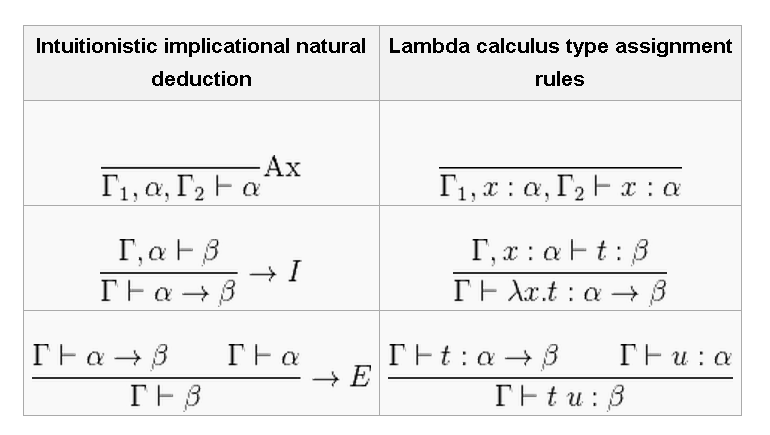
\includegraphics[width=11cm]{pics/curryhoward.png}



What we have seen so far leaves us with a new perspective on computation. No matter what language we choose, there seems to be a hard limit on what is possible to compute. This means that:

\begin{inparaenum}[\itshape i\upshape)]
\item programming languages all represent, at their core, the same set of objects (the set of all programs);
\item some problems cannot be solved with an automated solution, independently of the programming language;
\end{inparaenum}

Why is the search for new programming languages interesting thus, if they allow us no more expressive power? In reality, programming languages have more or less expressive power, but not because of what they can compute, but because they allow a clearer interaction with the \textit{humans} that use them. As A. Whitehead\footnote{A famous mathematician for as far as fame goes for mathematicians.} said in ``The Importance of Good Notation'', in his book \textit{An Introduction to Mathematics}:

\begin{displayquote}
[...] by the aid of symbolism, we can make transitions in reasoning almost mechanically by the eye, which otherwise would call into play the higher faculties of the brain.

[...]

One very important property for symbolism to possess is that it should be concise, so as to be visible at one glance of the eye and to be rapidly written. 

[...]

It is interesting to note how important for the development of science a modest-looking symbol may be. It may stand for the emphatic presentation of an idea, often a very subtle idea, and by its existence make it easy to exhibit the relation of this idea to all the complex trains of ideas in which it occurs. For example, take the most modest of all symbols, namely, 0, which stands for the number zero. The Roman notation for numbers had no symbol for zero, and probably most mathematicians of the ancient world would have been horribly puzzled by the idea of the number zero. For, after all, it is a very subtle idea, not at all obvious. A great deal of discussion on the meaning of the zero of quantity will be found in philosophic works. Zero is not, in real truth, more difficult or subtle in idea than the other cardinal numbers.
\end{displayquote}

Thus programming languages make it easier to express some aspects of thoughts rather than some others, and by emphasizing concepts such as correctness or reliability we can dramatically change the impact of the language on the thought process of the programmer.


About the unsolvable problem, also here is some silver present. Even though we cannot provide a perfect solution to these problems, nothing forbids us from building partial solutions that allow for uncertainty. We can thus always build a program that can answer questions about termination, correctness, or equivalence between programs with answers taken from the set \texttt{yes}, \texttt{no}, and \texttt{unknown}. The ability to return \texttt{unknown} suddenly makes the program possible to build, therefore exchanging some precision with implementability. 

The challenge that arises from this is thus that of reducing the number of programs for which our analyser returns \texttt{unknown} so that it is as small as possible. Not only do we wish to reduce the number of uncertain programs, we might also find it acceptable to have our analysis ``give up'' for programs where the flow of control is complex or hard to follow, in the assumptions that these programs, even when working, are not acceptable for being too confusing\footnote{If a program is confusing for a carefully built analyser, imagine what it does to the brain of Bob, a 20-something junior programmer who just came out of a coding bootcamp and sits two cubicles over.}. Theoretical frameworks such as dependent types, model checking, and abstract interpretation (just to name a few) are written with the goal in mind of standardizing the concepts of approximated analysis of computer programs, precisely with the goal of providing an incomplete, but still useful, solution to problems such as halting.



\chapter{Conclusions}
The goal of this document was to make you acquainted with the concept of inference systems. You have learned various aspects of logic and inference system, which we used to give rise to definitions of concepts such as numbers, boolean expressions, etc. Thanks to this we have seen how logical inference is actually self-sufficient to define all sorts of well-known mathematical concepts, without having to either:

\begin{inparaenum}[\itshape i\upshape)]
\item introduce these complex as primitive concepts, therefore making our formalism ``heavier'';
\item give them up and try to not use them.
\end{inparaenum}

Defining mathematical concepts could have gone further into most existing known aspects of mathematics, but instead after a while we have taken another route: defining whole programming languages as instances of logical inference. As a stepping stone we have defined a series of useful helpers, which are data structures such as lists or binary search trees. Then we have gone further to the definition of a small, yet whole, programming language.

This long trip has shown us not only the power of logic as a foundational tool for both mathematics and programming, but it has also shown the great potential of our logic-based language in the definition of programming languages.



\begin{appendices}
\chapter{A not so small imperative language}
\input{tex/examples/ImperativeLanguage/intro}
\subsection{Evaluating a C-{}- program}
A C-{}- program will take as input an empty memory state and a list of expressions (or statements). We define then the following keywords:

\begin{lstlisting}
Keyword [] "$m" Dictionary Priority 300 Class SymbolTable
Keyword [SymbolTable] "nextTable" [TableList] Priority 10 Class TableList
Keyword [] "nilTable" [] Priority 500 Class TableList
Keyword [SymbolTable] "add" [Id Value] Priority 100 Class DictionaryOp
Keyword [SymbolTable] "lookup" [Id] Priority 100 Class DictionaryOp
Keyword [SymbolTable] "contains" [Id] Priority 100 Class DictionaryOp

Keyword [Expr] ";" [ExprList] Priority 5 Class ExprList
Keyword [] "nop" [] Priority 500 Class ExprList

Keyword [] "program" [SymbolTable ExprList] Priority 0 Class Program
\end{lstlisting}

\noindent
Evaluating a C-{}- program means evaluating a series of statements separated by ``;'' and update the list of symbol tables at each evaluation. We can build an evaluation rule which takes the current statement, evaluates it, and then recursively call itself on the rest of the program. The evaluation rule returns the list of the updated symbol tables and the value returned by the evaluation.

\begin{lstlisting}
Keyword [] "eval" [TableList Expr] Priority 0 Class RuntimeOp
Keyword [] "evalResult" [TableList Value] Priority 0 Class EvaluationResult
\end{lstlisting}

The list of values available in C-{}- are the following:

\begin{lstlisting}
Keyword [] "$i" [<<int>>] Priority 300 Class Value
Keyword [] "$d" [<<double>>] Priority 300 Class Value
Keyword [] "$s" [<<string>>] Priority 300 Class Value
Keyword [] "$b" [<<bool>>] Priority 300 Class Value
Keyword [] "$void" [] Priority 300 Class Value
\end{lstlisting}

Starting from the \texttt{program}, we call the evaluation function on the program code. The program evaluation returns the updated global symbol table. The value returned by the program evaluation is \texttt{void} because a program is made by a sequence of statements that alter the memory, but they do not return any result.

\begin{lstlisting}
eval (memory nextTable nilTable) code => evalResult (memory' nextTable nilTable) $void
------------------------------------------------------------
program memory code => memory'
\end{lstlisting}

\noindent
The evaluation rule for a list of statements is the following:

\begin{lstlisting}
eval tables a => evalResult tables' $void
eval tables' b => res
----------------------------------------
eval tables (a;b) => res

-------------------------------------------
eval tables nop => evalResult tables $void
\end{lstlisting}

\noindent
We evaluate the head of the list, which possibly returns a modified list of symbol tables and returns \texttt{void} (we are evaluating a statement). We stop when we find the end of the sequence of statements.

In the following sections we will implement the evaluation rules for all the possible statements in the language.

\subsection{Variable definition}
C-{}- requires that the variable is defined before assigning a value to it. We define an operator called \texttt{variable} which takes a type followed by an identifier. The type are keywords themselves:

\begin{lstlisting}
Keyword [] "t_int" [] Priority 500 Class Type
Keyword [] "t_double" [] Priority 500 Class Type
Keyword [] "t_string" [] Priority 500 Class Type
Keyword [] "t_bool" [] Priority 500 Class Type
\end{lstlisting}

\noindent
An identifier is a string marked with the unary operator \texttt{\$}:

\begin{lstlisting}
Keyword [] "$" [<<string>>] Priority 300 Class Id
\end{lstlisting}

\noindent
The rule for variable definition calls the rule for adding an element into the symbol table. The correct symbol table which must store the variable, according to the scoping rules defined above, is the symbol table of the current scope, which is the first element of the symbol table list. All the variables are initialize with the default value \texttt{\$void}.

\begin{lstlisting}
Keyword [SymbolTable] "defineVariable" [Id] Priority 300 Class MemoryOp

symbols defineVariable id => symbols'
---------------------------------------------------
eval (symbols nextTable tables) (variable t id) => evalResult (symbols' nextTable tables) $void


  symbols add id $void => symbols'
  -------------------------------------
  symbols defineVariable id => symbols'
\end{lstlisting}

\subsection{Variable assignment}
Variable assignment has the form \texttt{\$id = expression}. 

\begin{lstlisting}
Keyword [Id] "=" [Expr] Priority 10 Class Expr
\end{lstlisting}

\noindent
The left side of the assignment is called \textit{lvalue}, and in our language can be only a variable. The right side of the assignment is called \textit{rvalue} and can be an arithmetic expression, a boolean expression, or another variable. The evaluation rule must evaluate the expression, look up the variable \textbf{in the whole symbol table list} taking the first occurrence, and write the value in the table. Before that we have to write the evaluation rules for rvalues.

\subsubsection{Atomic values}
The simplest case of rvalues is an atomic value. Atomic values in C-{}- can be integer, double, string, or boolean values. \texttt{\$void} value cannot be assigned to variables, nor be an expression. The evaluation rules for atomic values simply return the values themselves, without altering the symbol tables:

\begin{lstlisting}
------------------------------------------------
eval tables ($i v) => evalResult tables ($i v)

-----------------------------------------------
eval tables ($d v) => evalResult tables ($d v)

-----------------------------------------------
eval tables ($s v) => evalResult tables ($s v)

-----------------------------------------------
eval tables ($b v) => evalResult tables ($b v)
\end{lstlisting}

\subsubsection{Arithmetic expression evaluation}

An arithmetic expression is a composition of the operators +,-,*,/ whose left and right arguments can be recursively arithmetic expressions, variables or integer and double values. For example $1 + 3 * 5 - 4 / 6$ is made of $+$ applied to $1$ and $3 * 5 - 4 / 6$ whose arguments are $3 * 5$ and $4 / 6$. The evaluation rule simply evaluates recursively the arguments of an arithmetic operators and then combine the results. We will just show the evaluation rules for integer expressions, the rules for double expressions are the same. Also it is shown the + operator for string, which outputs the concatenation of two strings.

\begin{lstlisting}
eval tables expr1 => evalResult tables' ($i val1)
eval tables' expr2 => evalResult tables'' ($i val2)
arithmeticResult := <<val1 + val2>>
----------------------------------------------------------------------
eval tables expr1 + expr2 => evalResult tables'' ($i arithmeticResult)

eval tables expr1 => evalResult tables' ($i val1)
eval tables' expr2 => evalResult tables'' ($i val2)
arithmeticResult := <<val1 - val2>>
----------------------------------------------------------------------
eval tables expr1 - expr2 => evalResult tables'' ($i arithmeticResult)

eval tables expr1 => evalResult tables' ($i val1)
eval tables' expr2 => evalResult tables'' ($i val2)
arithmeticResult := <<val1 * val2>>
----------------------------------------------------------------------
eval tables expr1 * expr2 => evalResult tables'' ($i arithmeticResult)

eval tables expr1 => evalResult tables' ($i val1)
eval tables' expr2 => evalResult tables'' ($i val2)
arithmeticResult := <<val1 / val2>>
----------------------------------------------------------------------
eval tables expr1 / expr2 => evalResult tables'' ($i arithmeticResult)

eval tables expr1 => evalResult tables' ($s val1)
eval tables' expr2 => evalResult tables'' ($s val2)
arithmeticResult := <<val1 + val2>>
----------------------------------------------------------------------
eval tables expr1 + expr2 => evalResult tables'' ($s arithmeticResult)
\end{lstlisting}

\subsubsection{Boolean expression evaluation}
Boolean expressions can be obtained by either combining boolean operators or by using numeric comparison operators. In what follows we will give the evaluation rules only for integer comparison operators, the rules for double values are analogous. Equality and inequality operators can be applied to any value.

\begin{lstlisting}
eval tables expr1 => evalResult tables' ($b val1)
eval tables' expr2 => evalResult tables'' ($b val2)
boolResult := <<val1 && val2>>
----------------------------------------------------------------------
eval tables expr1 && expr2 => evalResult tables'' ($b boolResult)

eval tables expr1 => evalResult tables' ($b val1)
eval tables' expr2 => evalResult tables'' ($b val2)
boolResult := <<val1 || val2>>
----------------------------------------------------------------------
eval tables expr1 || expr2 => evalResult tables'' ($b boolResult)


eval tables expr => evalResult tables' ($b val)
boolResult := << !val >>
--------------------------------------------------------
eval tables (!expr) => evalResult tables' ($b boolResult)

eval tables expr1 => evalResult tables' val1
eval tables' expr2 => evalResult tables'' val2
val1 == val2
--------------------------------------------------------
eval tables (expr1 equals expr2) => evalResult tables' ($b true)

eval tables expr1 => evalResult tables' val1
eval tables' expr2 => evalResult tables'' val2
val1 != val2
--------------------------------------------------------
eval tables (expr1 equals expr2) => evalResult tables' ($b false)


eval tables (expr1 equals expr2) => evalResult tables' ($b res)
boolResult := << !res >>
-------------------------------------------------------------------
eval tables (expr1 neq expr2) => evalResult tables' ($b boolResult)

eval tables expr1 => evalResult tables' ($i val1)
eval tables' expr2 => evalResult tables'' ($i val2)
boolResult := << val1 < val2 >>
---------------------------------------------------------
eval tables (expr1 ls expr2) => evalResult tables' ($b boolResult)

eval tables expr1 => evalResult tables' ($i val1)
eval tables' expr2 => evalResult tables'' ($i val2)
boolResult := << val1 <= val2 >>
---------------------------------------------------------
eval tables (expr1 leq expr2) => evalResult tables' ($b boolResult)

eval tables expr1 => evalResult tables' ($i val1)
eval tables' expr2 => evalResult tables'' ($i val2)
boolResult := << val1 > val2 >>
---------------------------------------------------------
eval tables (expr1 grt expr2) => evalResult tables' ($b boolResult)

eval tables expr1 => evalResult tables' ($i val1)
eval tables' expr2 => evalResult tables'' ($i val2)
boolResult := << val1 >= val2 >>
---------------------------------------------------------
eval tables (expr1 geq expr2) => evalResult tables' ($b boolResult)
\end{lstlisting}

\subsubsection{Variable lookup}
The last case of rvalue (and also of arithmetic and boolean expression) is the variable assignment. The rule must iterate the symbol table list until it finds a variable matching the variable name. Then it returns the value contained in that variable.

\begin{lstlisting}
symbols contains ($name) => Yes
symbols lookup ($name) => val
-----------------------------------------------------------
eval (symbols nextTable tables) ($name) => evalResult (symbols nextTable tables) val


symbols contains ($name) => No
eval tables ($name) => evalResult tables' val
-----------------------------------------------------------
eval (symbols nextTable tables) ($name) => evalResult (symbols nextTable tables') val
\end{lstlisting}

\subsubsection{Evaluation of the assignment}
One could be prone to write the following rules for the assignment:

\begin{lstlisting}
table contains id => Yes
eval table expr => evalResult table' val
table add id val => table''
-------------------------------------------------------
eval (table nextTable tables) (id = expr) => evalResult table'' 

table contains id => No
eval tables (id = expr) => res
---------------------------------------------------------
eval (table nextTable tables) (id = expr) => res
\end{lstlisting}

\noindent
If the lvalue is contained in the current symbol table we update it with the result of the expression evaluation, otherwise we iterate the symbol table list. This implementation is however \textbf{wrong}. Indeed consider the assignment \texttt{z = z + y} in the example using variable scoping in Section \ref{sec:semantics}. The variable \texttt{z} is not in the current scope symbol table, so we recursively call \texttt{eval} dropping the head of the list. At this point we have a symbol table which contains \texttt{z}. Unfortunately, when we evaluate the rvalue, we cannot find \texttt{y} which was in the symbol table we dropped before the recursive call.

From this example we see that we need to keep the original list of symbol tables to be able to perform the correct lookup for rvalues. We rewrite the evaluation rule using a different rule \texttt{updateTables} which correctly perform the assignment by carrying both the current scope list and the original list with all the symbol tables.

\begin{lstlisting}
symbols contains id => Yes
eval globals expr => evalResult globals' val
symbols add id val => symbols'
-------------------------------------------------------
updateTables globals (symbols nextTable tables) id expr => evalResult (symbols' nextTable tables) $void 

symbols contains id => No
updateTables globals tables id expr => evalResult tables' $void
-------------------------------------------------------
updateTables globals (symbols nextTable tables) id expr => evalResult (symbols nextTable tables') $void


updateTables tables tables id expr => res
----------------------------------------
eval tables (id = expr) => res
\end{lstlisting}

\noindent
The new rule evaluates the rvalue by using the global table instead of the partial symbol table carried by the recursive calls, so that it can correctly access all the variables defined so far.

\subsection{Evaluation of the If-Else statement}
This statement has the form \texttt{if (condition) then expr1 else expr2}.

\begin{lstlisting}
Keyword [] "then" [] Priority 10 Class Then
Keyword [] "else" [] Priority 10 Class Else
Keyword [] "if" [Expr Then Expr Else Expr] Priority 10 Class Expr
\end{lstlisting}

\noindent
The operational semantics is that if the boolean expression in the condition evaluates \texttt{true} we evaluate \texttt{expr1} otherwise we evaluate \texttt{expr2}. When we execute either of the two blocks, we have to add a symbol table for the scope of the new body we are going to evaluate. When the body has been evaluated, we discard the symbol table we added (because we are exiting the \texttt{if-else} scope) and keep the other possibly modified symbol tables. Thus we have two evaluation rules:

\begin{lstlisting}
eval tables condition => evalResult tables' ($b true)
eval (empty nextTable tables) expr1 => evalResult (table' nextTable tables'') val
-----------------------------------------------------
eval tables (if condition then expr1 else expr2) => evalResult tables'' val

eval tables condition => evalResult tables' ($b false)
eval (empty nextTable tables) expr2 => evalResult (table' nextTable tables'') val
-----------------------------------------------------
eval tables (if condition then expr1 else expr2) => evalResult tables'' val
\end{lstlisting}

\subsection{Evaluation of the While statement}
This statement has the form \texttt{while (condition) expr}

\begin{lstlisting}
Keyword [] "while" [Expr Expr] Priority 10 Class Expr
\end{lstlisting}

The statement evaluates the condition, then executes \texttt{expr} if the condition is true. At the end of the body evaluation we re-evaluate the condition and possibly execute the body again. If the condition is false we skip to the next statement. The considerations about the symbol tables done for the \texttt{if-else} statement are the same:

\begin{lstlisting}
eval tables condition => evalResult tables' ($b true)
eval (empty nextTable tables) expr => evalResult (table' nextTable tables'') val
eval tables'' (while condition expr) => res
---------------------------------------------------
eval tables (while condition expr) => res

eval tables condition => evalResult tables' ($b false)
-----------------------------------------------------------
eval tables (while condition expr) => evalResult tables' $void
\end{lstlisting}

\subsection{Evaluation of the For statement}
This statement has the form \texttt{for (init condition step) expr}

\begin{lstlisting}
Keyword [] "for" [Expr Expr Expr Expr] Priority 10 Class Expr
\end{lstlisting}

\noindent
The statement evaluates once the \texttt{init} statement. After that it evaluates the condition, and if it is true \texttt{expr} is evaluated. At the end of the evaluation the \texttt{step} statement is evaluated and then the condition is evaluated again.

Since the \texttt{init} statement must be executed only once, we cannot recursively call the evaluation rule for the \texttt{for} statement directly. We then define a keyword \texttt{loopFor} which do the evaluations after the \texttt{init} statement has been evaluated.

\noindent
\begin{lstlisting}
Keyword [] "loopFor" [TableList Expr Expr Expr] Priority 0 Class RuntimeOp
\end{lstlisting}

\noindent
The rule associated to this keyword evaluates the condition and the body, updating the symbol tables accordingly.
\begin{lstlisting}
eval tables init => evalResult tables' $void
loopFor tables' condition step expr => res
-------------------------------------------------------
eval tables (for init condition step expr) => res

  eval tables condition => evalResult tables' ($b true)
  eval (empty nextTable tables) expr => evalResult (table' nextTable tables'') val
  eval tables'' step => evalResult tables3 val'
  loopFor tables3 condition step expr => res 
  ------------------------------------------------------------------
  loopFor tables condition step expr => res

  eval tables condition => evalResult tables' ($b false)
  ------------------------------------------------------------------
  loopFor tables condition step expr => evalResult tables' $void
\end{lstlisting}
The goal of this document was to make you acquainted with the concept of inference systems. You have learned various aspects of logic and inference system, which we used to give rise to definitions of concepts such as numbers, boolean expressions, etc. Thanks to this we have seen how logical inference is actually self-sufficient to define all sorts of well-known mathematical concepts, without having to either:

\begin{inparaenum}[\itshape i\upshape)]
\item introduce these complex as primitive concepts, therefore making our formalism ``heavier'';
\item give them up and try to not use them.
\end{inparaenum}

Defining mathematical concepts could have gone further into most existing known aspects of mathematics, but instead after a while we have taken another route: defining whole programming languages as instances of logical inference. As a stepping stone we have defined a series of useful helpers, which are data structures such as lists or binary search trees. Then we have gone further to the definition of a small, yet whole, programming language.

This long trip has shown us not only the power of logic as a foundational tool for both mathematics and programming, but it has also shown the great potential of our logic-based language in the definition of programming languages.

\end{appendices}


\end{document}
